\documentclass[10pt,a4paper,oneside]{report}

\usepackage[section] {placeins}

\usepackage[norsk,english]{babel}
\usepackage[utf8]{inputenc}
\usepackage[T1]{fontenc}

\selectlanguage{english}

\usepackage{graphicx}
\usepackage{tabularx}
\usepackage{booktabs}
\usepackage{wrapfig}
\usepackage{pbox}

\usepackage{fullpage}
\usepackage{verbatim}
\usepackage{url}

\usepackage[section]{placeins}

\fontfamily{ptm}\selectfont

\usepackage{hyperref}
\hypersetup{
    bookmarks=true,
    unicode=true,
    pdftoolbar=true,
    pdfmenubar=true,
    pdffitwindow=false,
    pdfstartview={FitH},
    pdftitle={Wonsole Administrator Manual},
    pdfauthor={Ivo DLouhy},
    pdfsubject={Wonsole User Manual},
    %pdfcreator={Creator},
    %pdfproducer={Producer},
    pdfkeywords={ntnu} {customer-driven-project} {wonsole} {manual},
    pdfnewwindow=true,
    colorlinks=true,
    linkcolor=blue,
    citecolor=red,
    filecolor=blue,
    urlcolor=blue
}


\bibliographystyle{plain}

\begin{document}

\thispagestyle{empty}
\begin{center}
	\vspace{\stretch{0.7}}
	{\Huge Wonsole} \\
	\medskip
	{\LARGE The new web console for power users} \\ 
	\bigskip
	{\Huge User Manual} \\ 
	\vspace{\stretch{0.3}}
	
\includegraphics[width=2.5in]{image/logo-ntnu.pdf} \\
	
\includegraphics[width=2.5in]{image/logo-netlight.png}
\end{center}
{\Large \textsc{Customer Driven Project}} \\
{\large \today \\Team: Ivo Dlouhy, Martin Havig, Øystein Heimark, Oddvar Hungnes}
\newpage

\setcounter{tocdepth}{1}
\tableofcontents
\clearpage
\listoffigures


\chapter{Introduction}
This document describes how to use the Wonsole application. It contains a user
tutorial as well as command refence.

\chapter{Basics}
User interface for wonsole is minimal a simple, so that the funcionality gets
presented in a clear way. If you see the main screen in the
picture \ref{wonsole2-00}, on the left hand side, there is a GUI - Graphical
User Interface - this is where data get presented as graphics. On the right hand side, there is a console window. This is a place
where user can input the commands and send the commands to the system by
pressing enter.

By default the list of available databases is displayed in GUI and
command prompt in console.


\begin{figure}
\centering
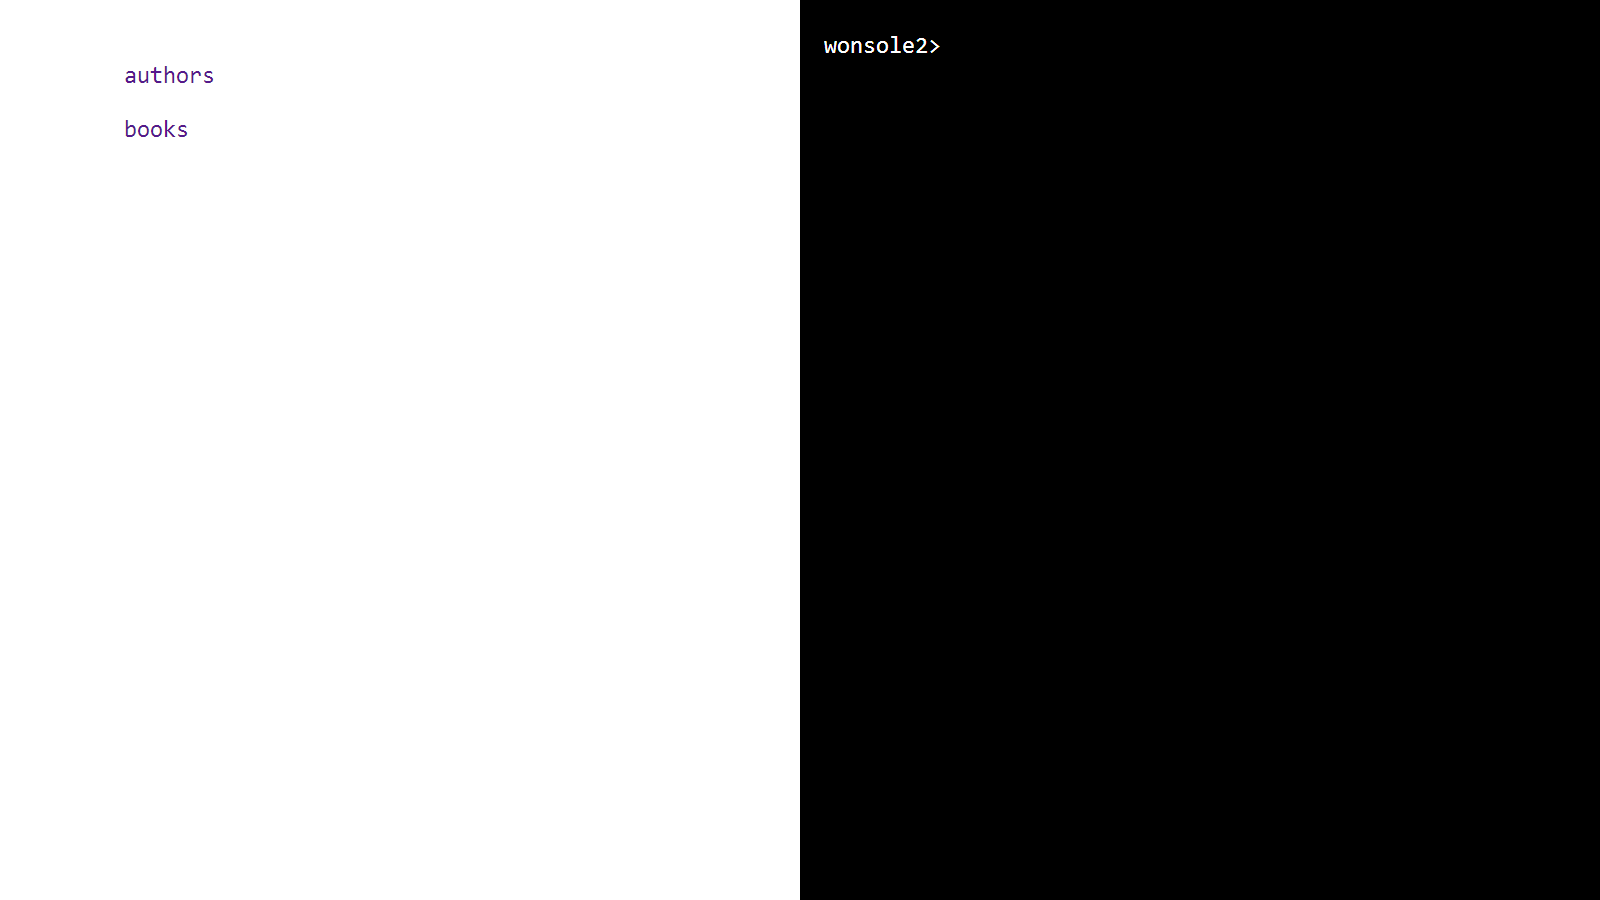
\includegraphics[width=\textwidth]{screenshot/wonsole2/wonsole2-00.png}
\caption{Main screen}
\label{wonsole2-00}
\end{figure}

\chapter{Tutorial}

\section{Database}
The most basic command in Wonsole is the command to open, or switch database. It
has this format:
\begin{verbatim}
db DATABASE
\end{verbatim}
Where DATABASE is the name of the database to open. Databases are listed in GUI
and they can be opened by clicking at the name too.

After issuing the command, the database contents are displayed in GUI, see
picture \ref{wonsole2-02}.
Wonsole uses document oriented database, so it is list of documents indexed by numbers.
From each document the title attribute is displayed as preview.


\begin{figure}
\centering
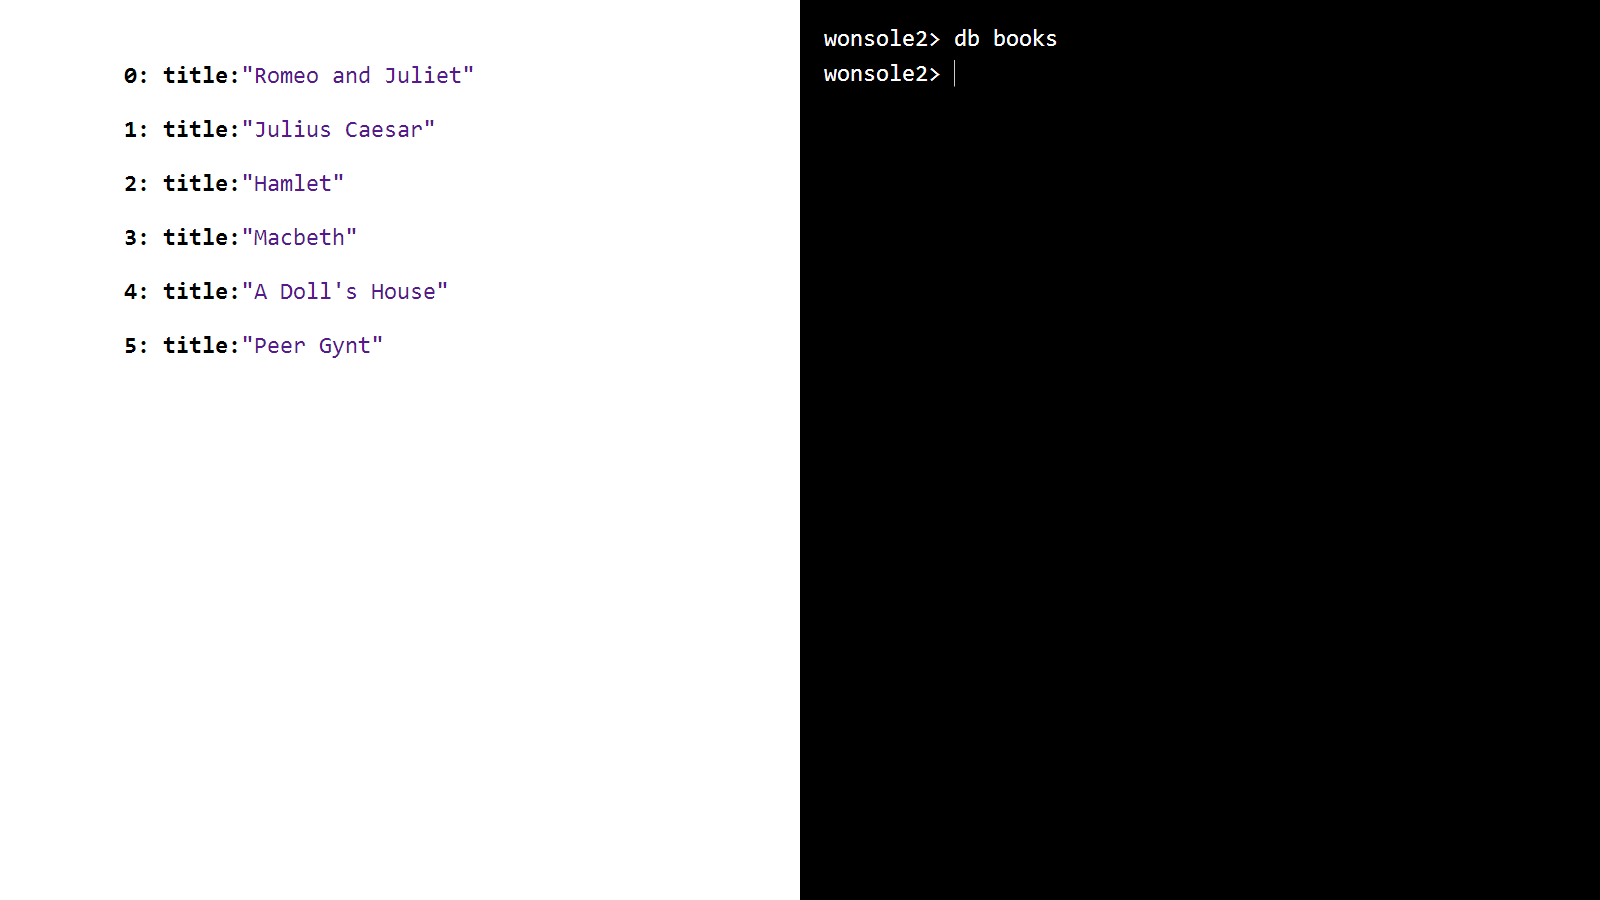
\includegraphics[width=\textwidth]{screenshot/wonsole2/wonsole2-02.png}
\caption{Database open}
\label{wonsole2-02}
\end{figure}

Same command can be used to switch the database anywhere in the workflow as in
picture \ref{wonsole2-04}.

\textit{Note: All uncommited changes are lost when switching the database.}

\begin{figure}
\centering
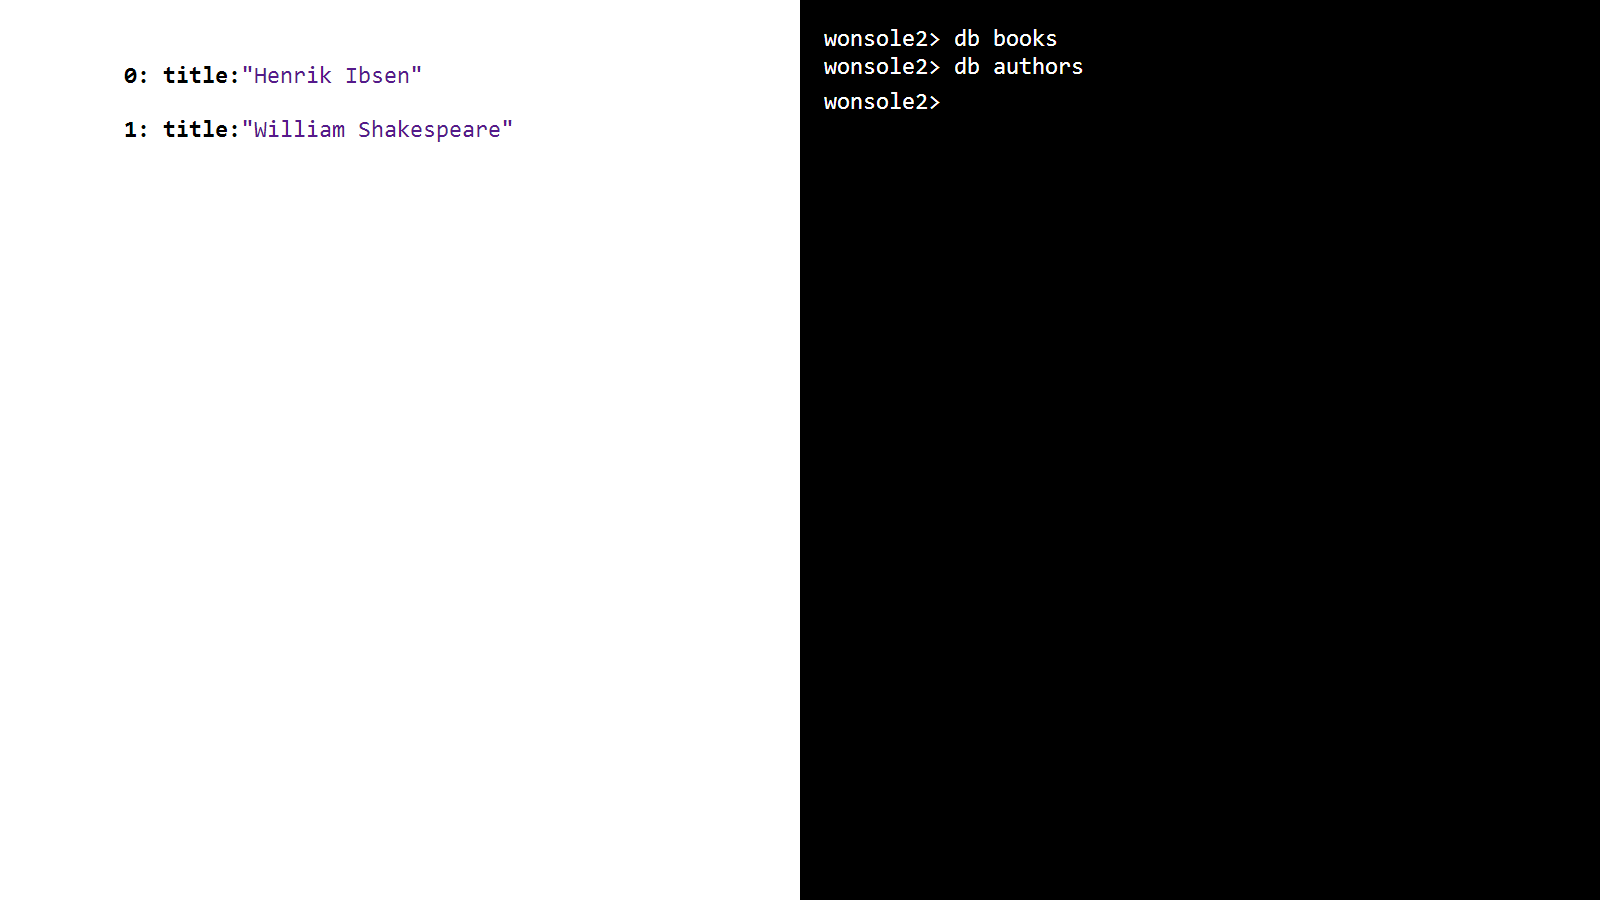
\includegraphics[width=\textwidth]{screenshot/wonsole2/wonsole2-04.png}
\caption{Database switch}
\label{wonsole2-04}
\end{figure}

\section{Log}
\textit{Note: Developers only.}

\section{Print}
Command print is available to display data in plaintext instead of using GUI.
It's syntax is very simple - it has one attribute: variable or data to print.
\begin{verbatim}
print DATA
\end{verbatim}
Command loads the data, converts it into text and prints in the console as ssen
in picture \ref{wonsole2-10}.

\begin{figure}
\centering
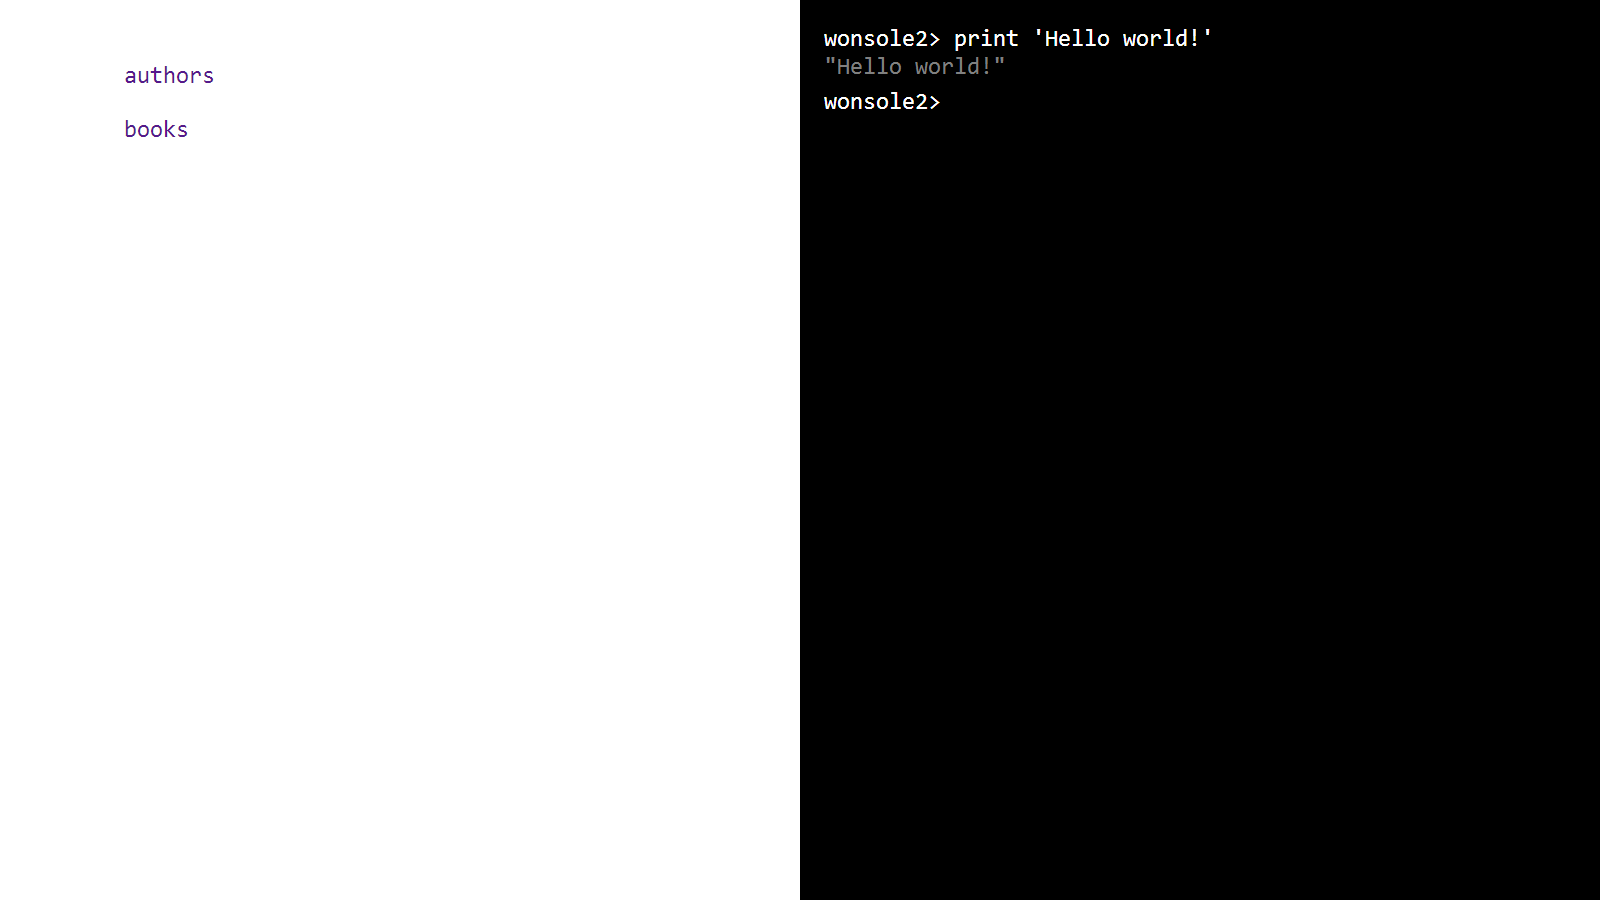
\includegraphics[width=\textwidth]{screenshot/wonsole2/wonsole2-10.png}
\caption{Print}
\label{wonsole2-10}
\end{figure}



\section{View}
Oposite of the print command there is view. It displays the complex variable in
the GUI.
\begin{verbatim}
view VARIABLE
\end{verbatim}


\chapter{Appendices}
\section{Command reference}
%\begin{verbatim}

\begin{table}
\centering
\begin{tabularx}{\textwidth}{ | l | X | l | }
\hline
\textbf{command} & \textbf{description} & \textbf{example} \\ \hline 
db DATABASE	& opens database DATABASE & db books \\ \hline
docs & switches view to documents & docs \\ \hline
doc INDEX & opens document at INDEX & doc 0 \\ \hline
commit & commits the changes to database & commit \\ \hline
rollback & rollbacks the changes & rollback \\ \hline
refresh & refreshes the UI & refresh \\ \hline
clear & clears the console & clear \\ \hline
print & VARIABLE	prints the variable VARIABLE & print docs \\ \hline
quiet & toggles list verbosity, default: on & quiet \\ \hline
log & toggles log visibility, default: off & log \\ \hline
remove INDEX & removes object at index INDEX & remove 0 \\ \hline
remove JSON & removes object specified by JSON & remove  \{"id":1231232\} \\ \hline
add JSON & adds object specified by JSON & add \{"title" : "New book"\} \\ \hline
seteach ARRAY ATTRIBUTE VALUE & sets (creates if necessary) ATTRIBUTE in object in ARRAY to VALUE & seteach docs author "Unknown" \\ \hline
foreach ARRAY CODE & executes the CODE for each item of ARRAY & foreach docs price=price*10 \\ \hline
filter ARRAY ATTRIBUTE VALUE & filters the ARRAY with VALUE of ATTRIBUTE & filter docs  title Report \\ \hline
script ARRAY & executes the ARRAY of commands specified by string & script ["clear", "db books"] \\ \hline
\end{tabularx}
\caption{Command reference}
\label{table:command-reference}
\end{table}
%\end{verbatim}




%\chapter{screenshots}
%\centering
\begin{figure}
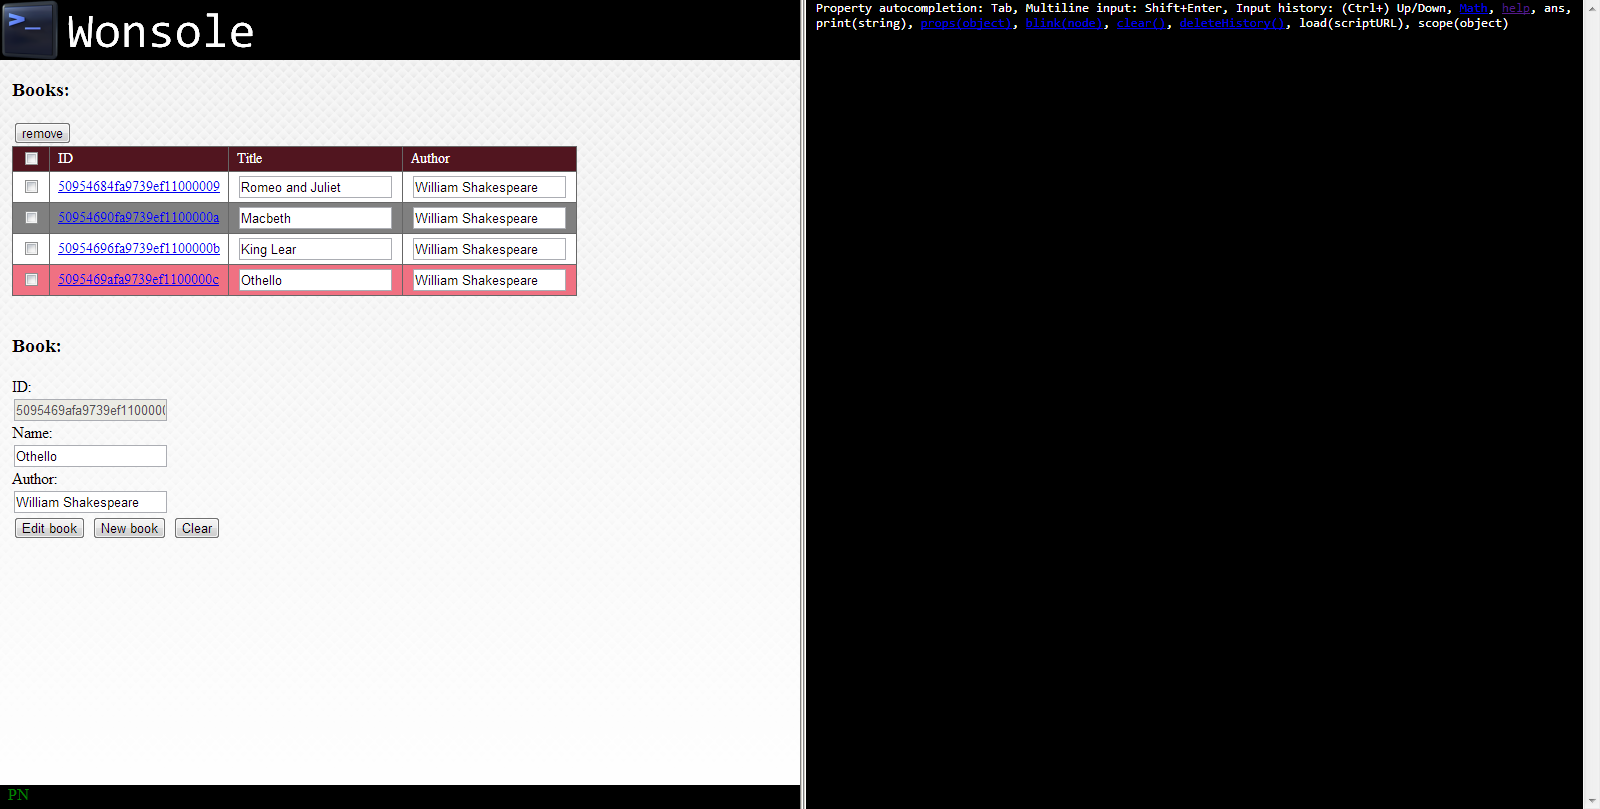
\includegraphics[width=\textwidth]{screenshot/wonsole1-01-initial.png}
\caption{wonsole1-01-initial.png}
\label{wonsole1-01-initial.png}
\end{figure}


\begin{figure}
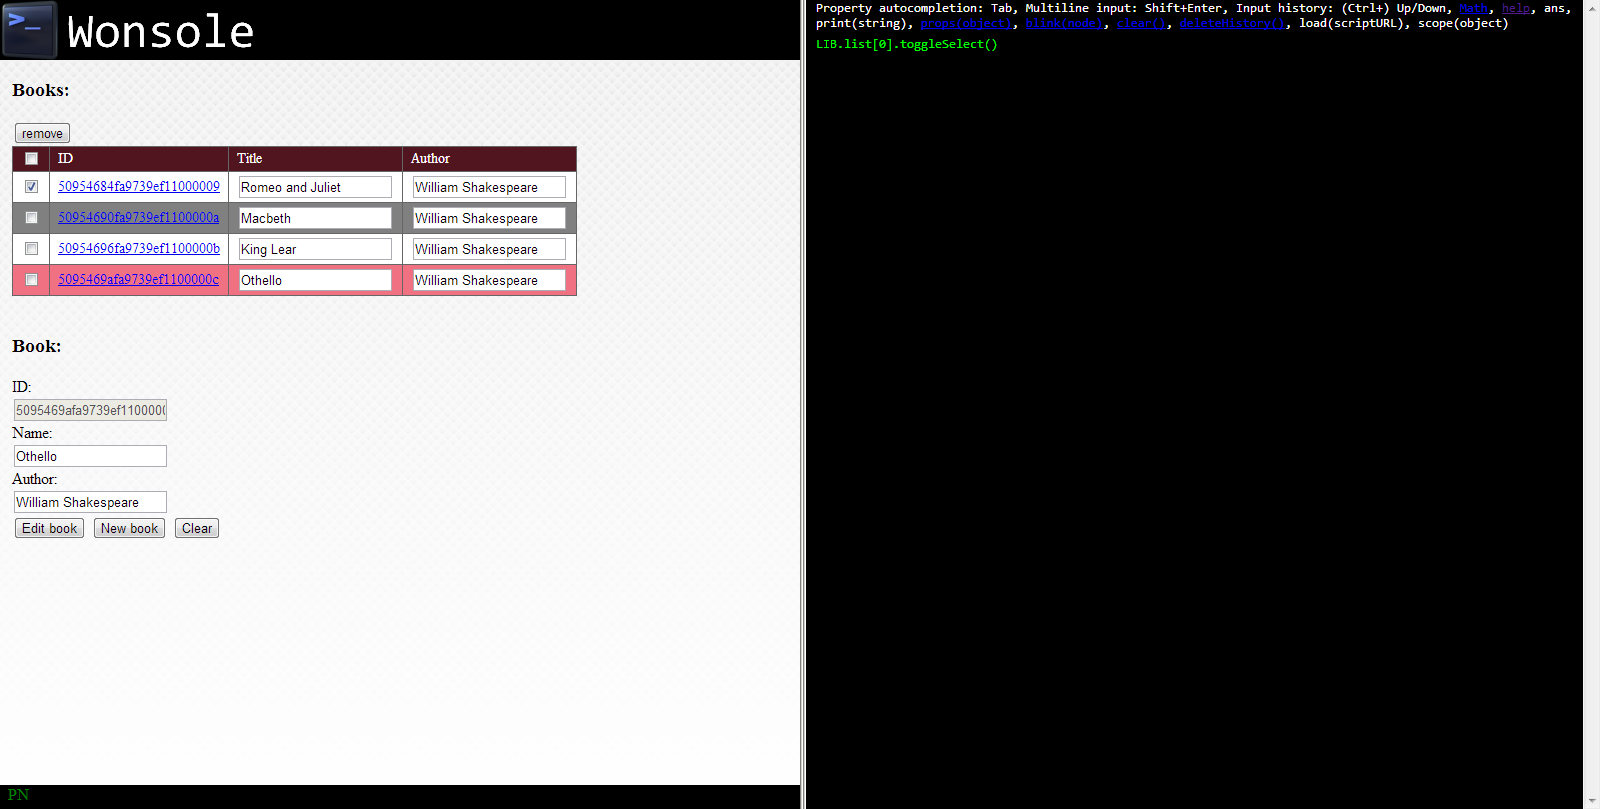
\includegraphics[width=\textwidth]{screenshot/wonsole1-02-gui-select.png}
\caption{wonsole1-02-gui-select.png}
\label{wonsole1-02-gui-select.png}
\end{figure}


\clearpage
\begin{figure}
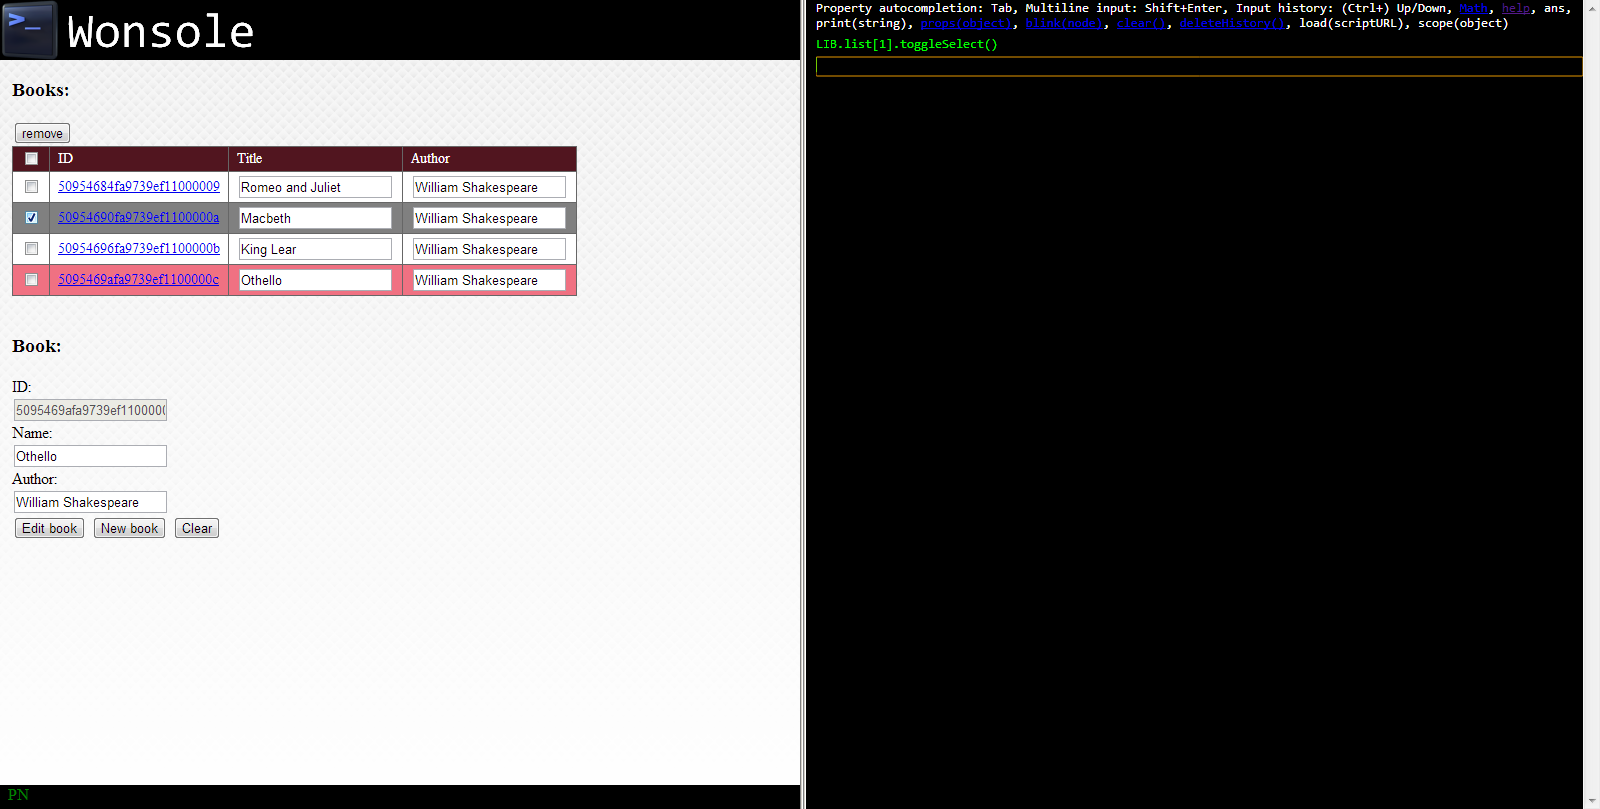
\includegraphics[width=\textwidth]{screenshot/wonsole1-03-gui-select.png}
\caption{wonsole1-03-gui-select.png}
\label{wonsole1-03-gui-select.png}
\end{figure}


\begin{figure}
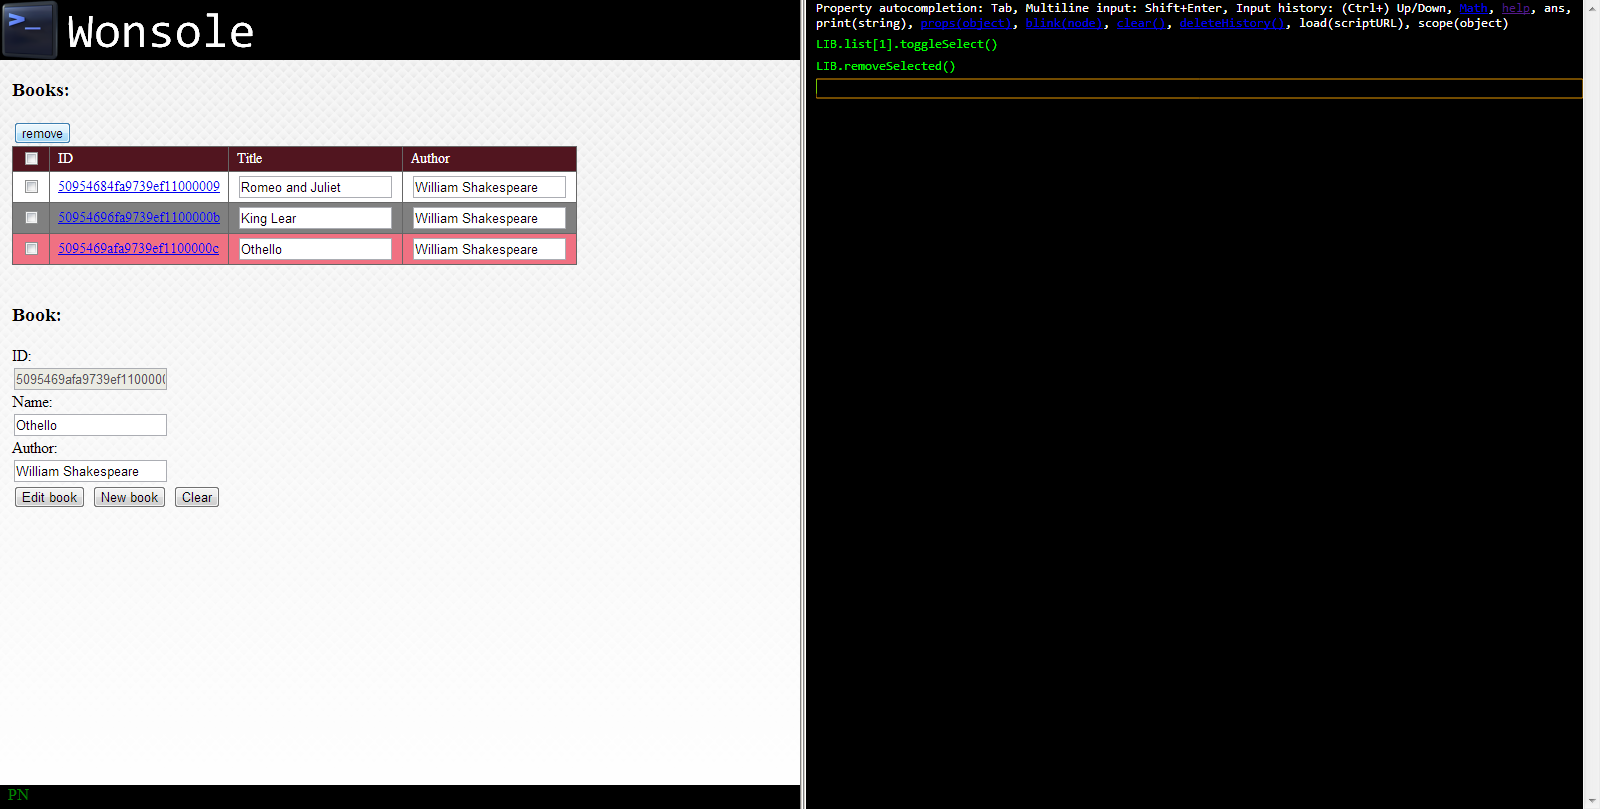
\includegraphics[width=\textwidth]{screenshot/wonsole1-04-gui-remove-selected.png}
\caption{wonsole1-04-gui-remove-selected.png}
\label{wonsole1-04-gui-remove-selected.png}
\end{figure}


\clearpage
\begin{figure}
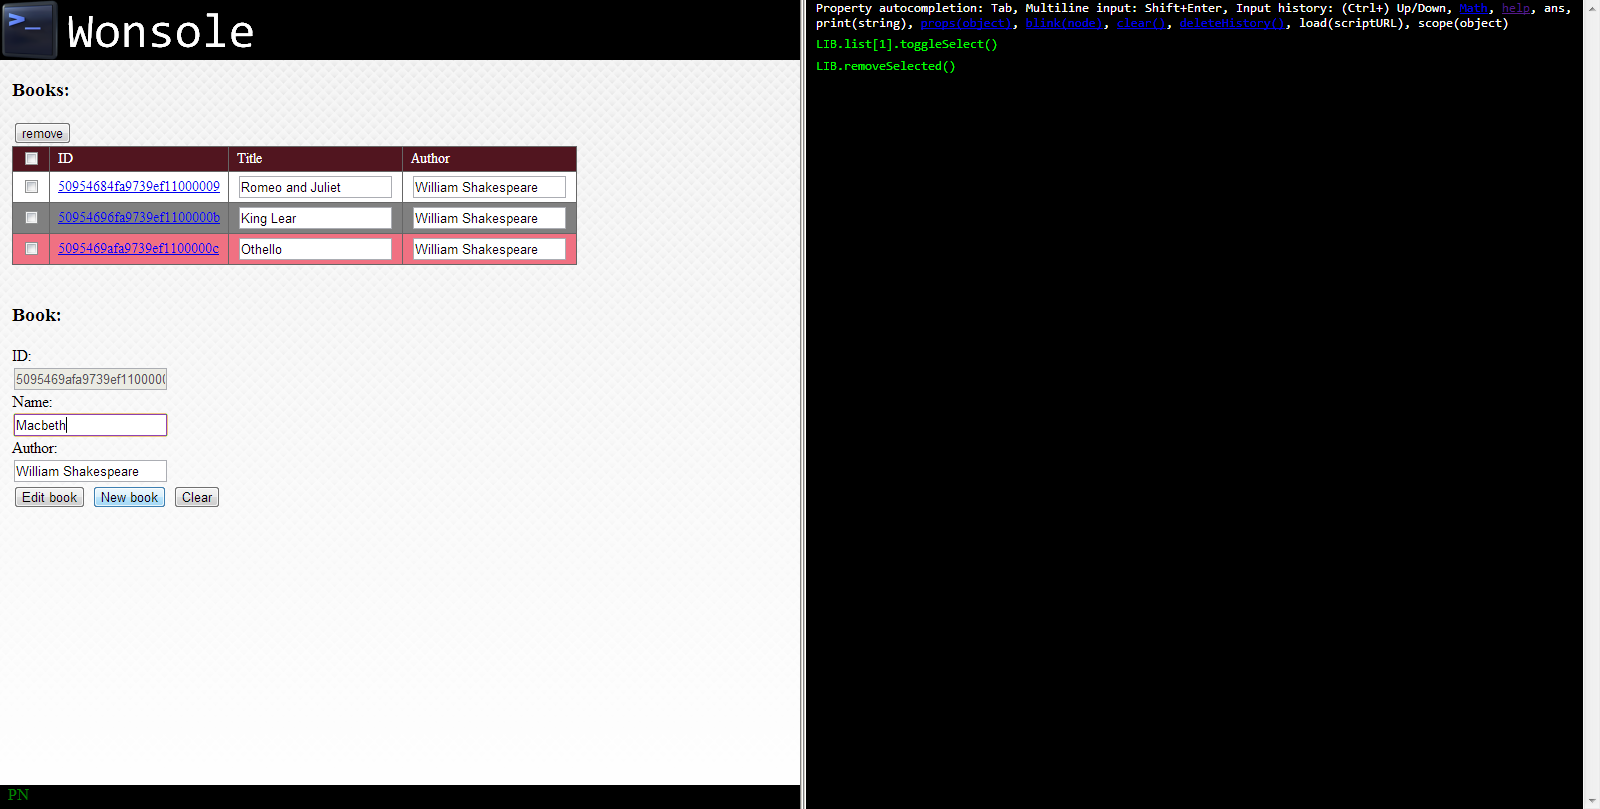
\includegraphics[width=\textwidth]{screenshot/wonsole1-05-gui-add-form.png}
\caption{wonsole1-05-gui-add-form.png}
\label{wonsole1-05-gui-add-form.png}
\end{figure}


\begin{figure}
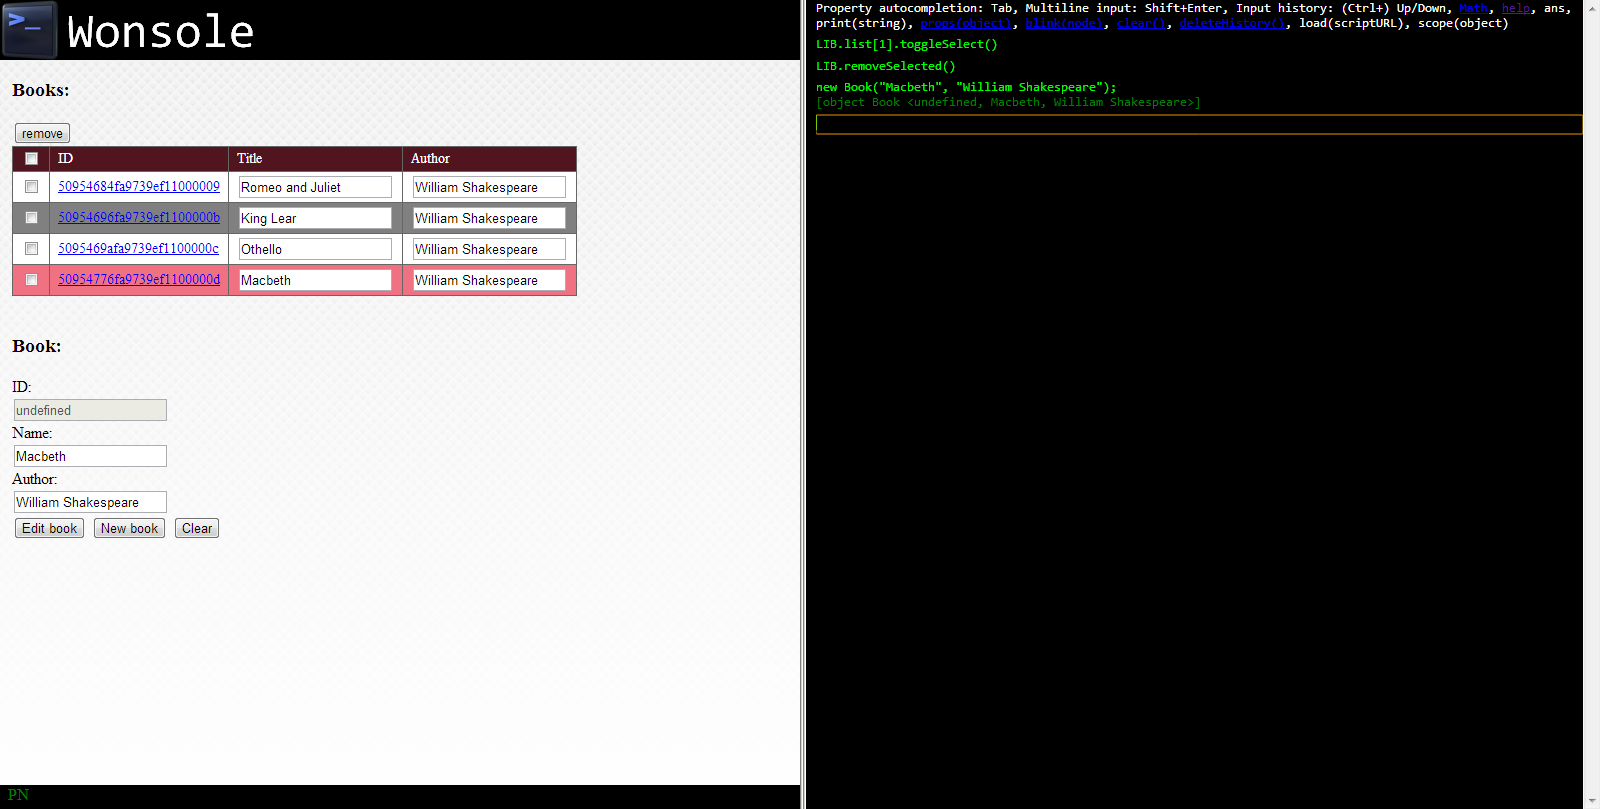
\includegraphics[width=\textwidth]{screenshot/wonsole1-06-gui-add-submit.png}
\caption{wonsole1-06-gui-add-submit.png}
\label{wonsole1-06-gui-add-submit.png}
\end{figure}


\clearpage
\begin{figure}
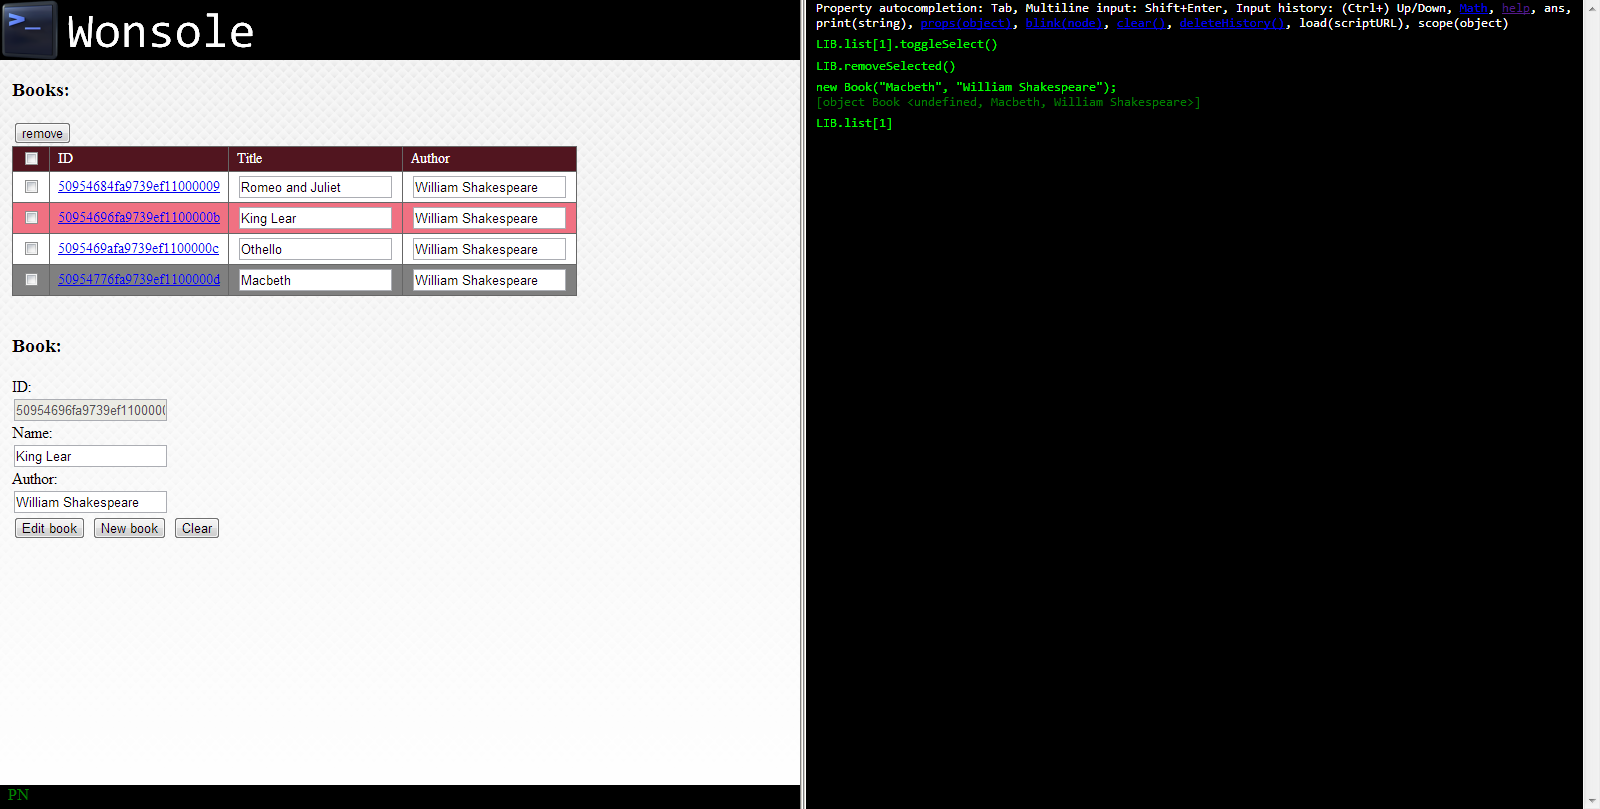
\includegraphics[width=\textwidth]{screenshot/wonsole1-07-gui-select.png}
\caption{wonsole1-07-gui-select.png}
\label{wonsole1-07-gui-select.png}
\end{figure}


\begin{figure}
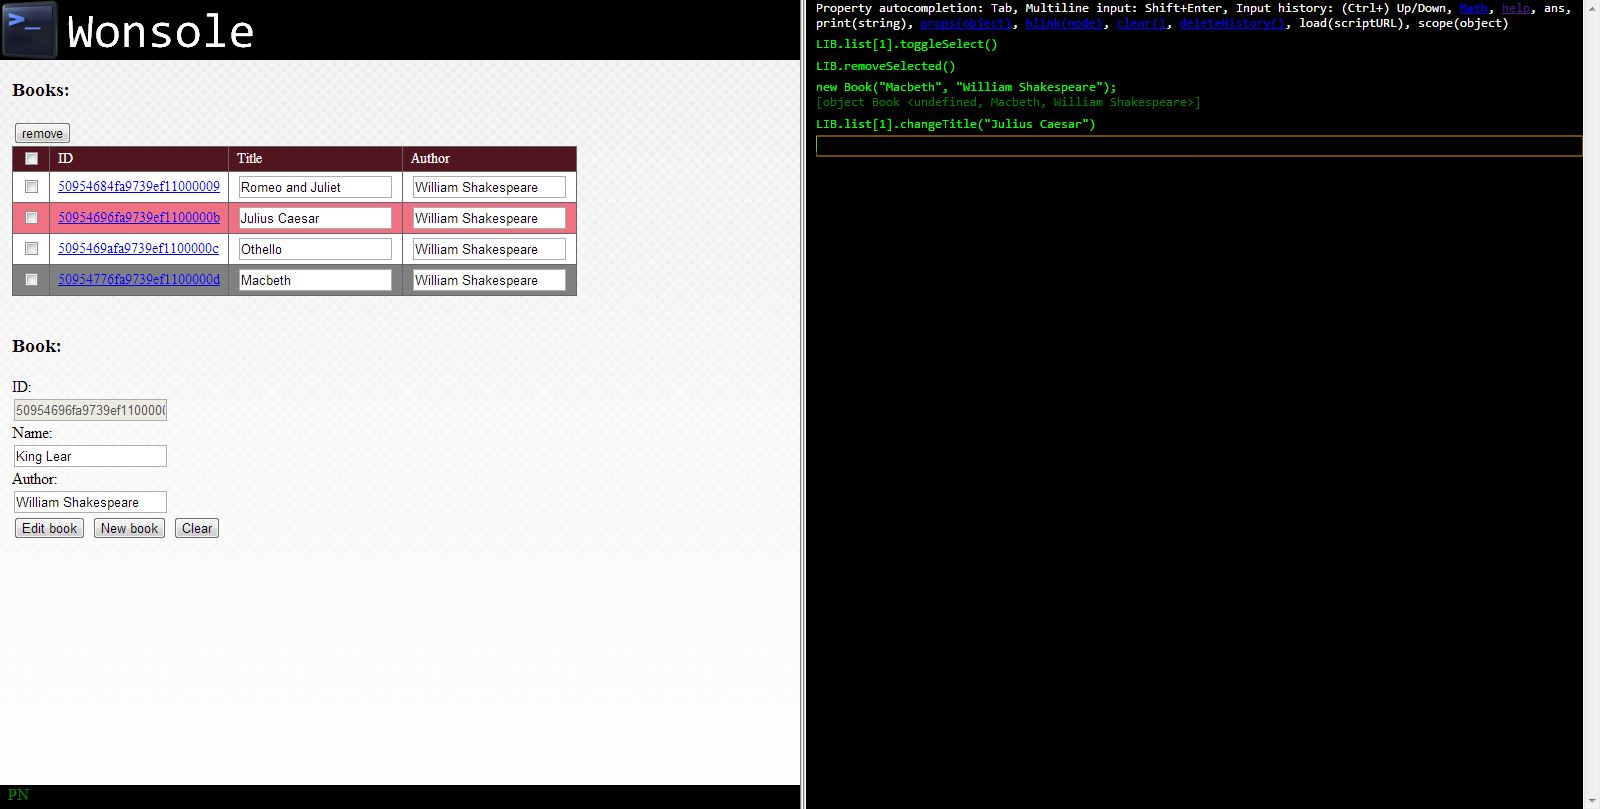
\includegraphics[width=\textwidth]{screenshot/wonsole1-08-gui-rename.png}
\caption{wonsole1-08-gui-rename.png}
\label{wonsole1-08-gui-rename.png}
\end{figure}


\clearpage
\begin{figure}
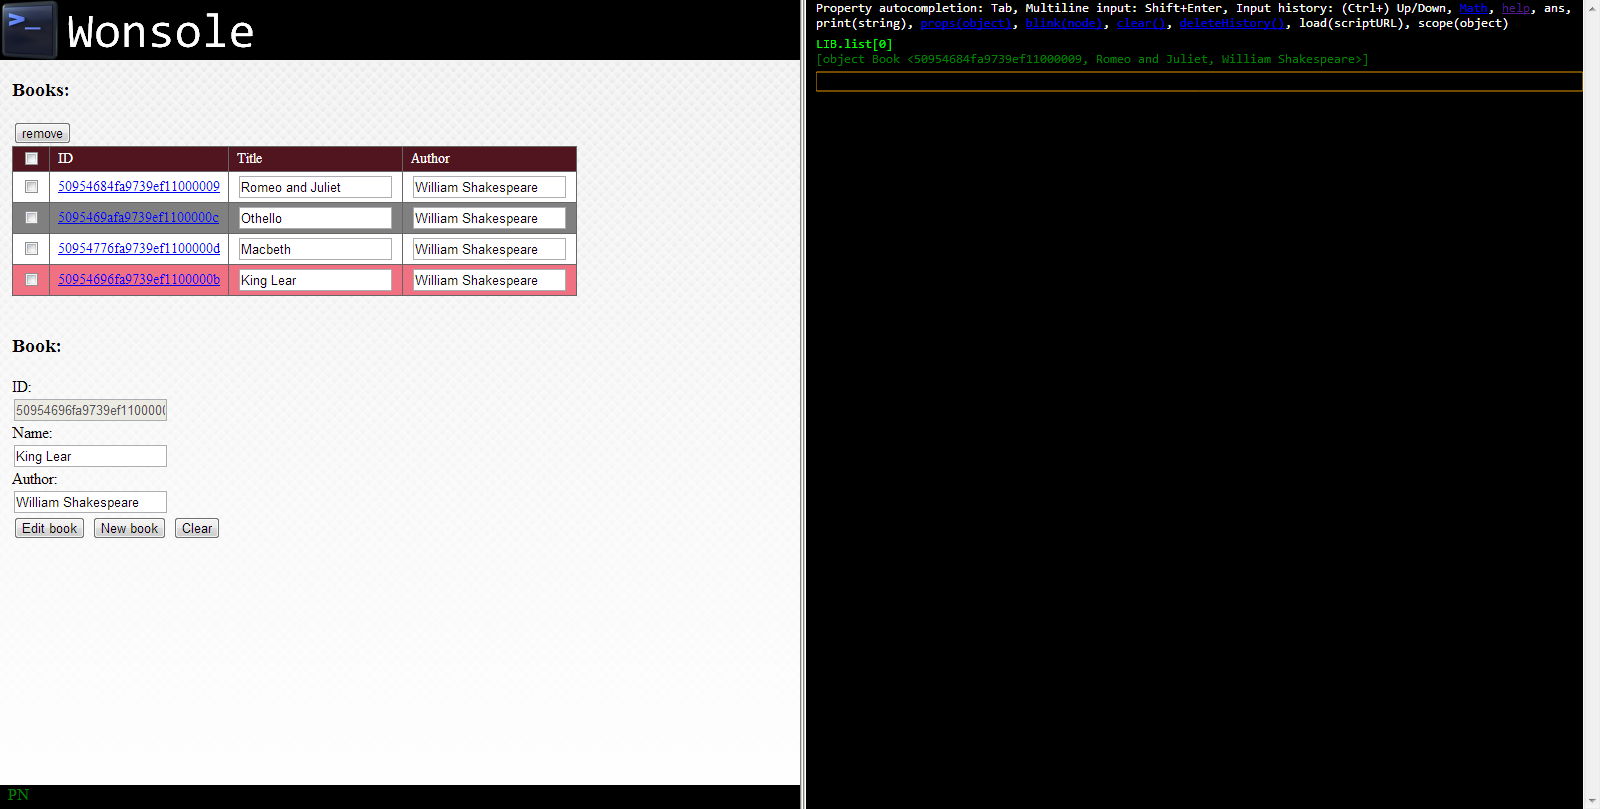
\includegraphics[width=\textwidth]{screenshot/wonsole1-09-list.png}
\caption{wonsole1-09-list.png}
\label{wonsole1-09-list.png}
\end{figure}


\begin{figure}
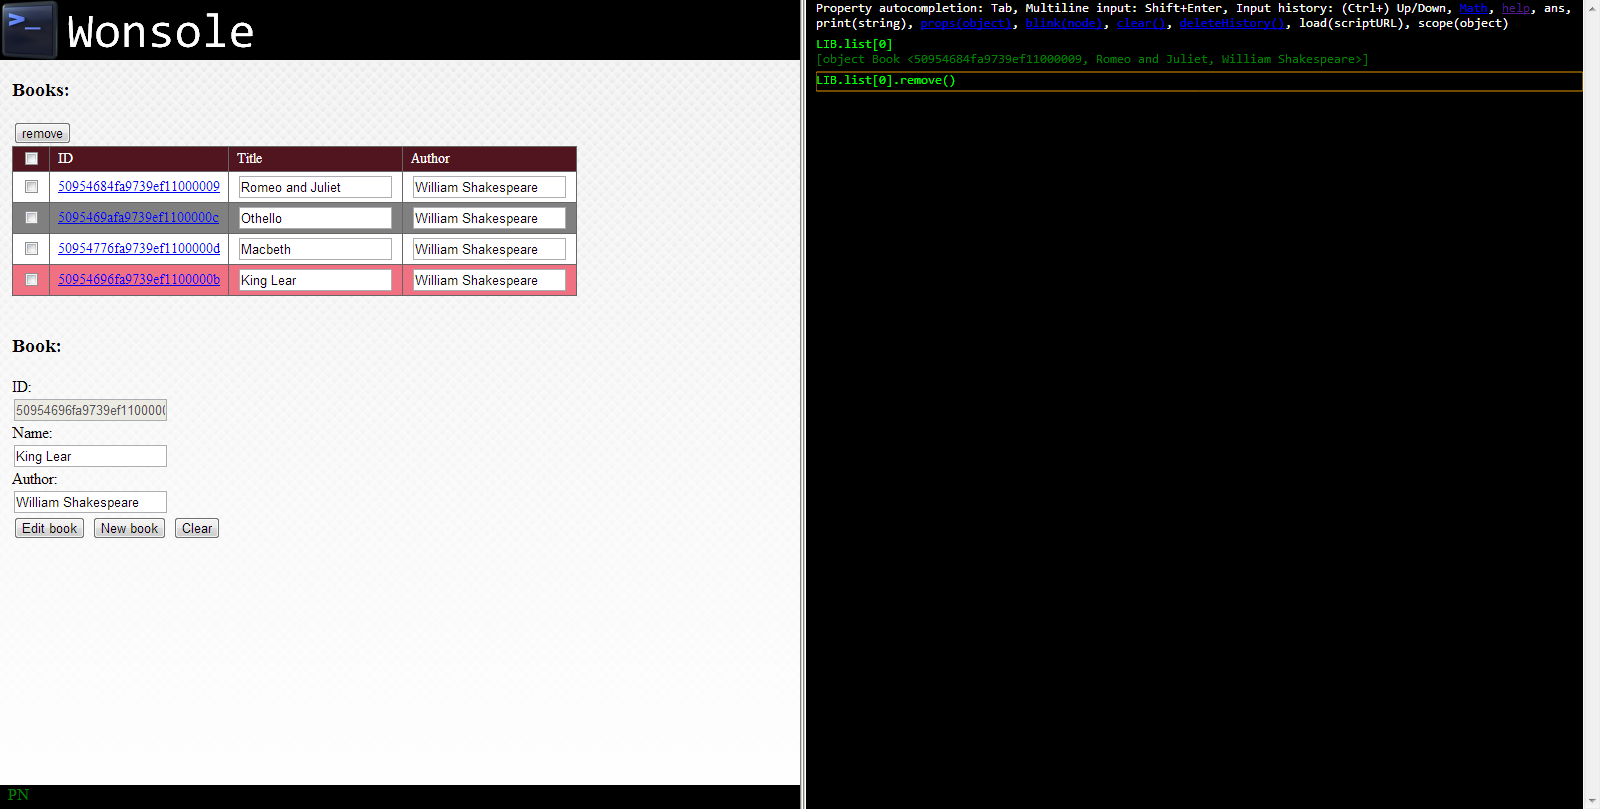
\includegraphics[width=\textwidth]{screenshot/wonsole1-10-delete.png}
\caption{wonsole1-10-delete.png}
\label{wonsole1-10-delete.png}
\end{figure}


\clearpage
\begin{figure}
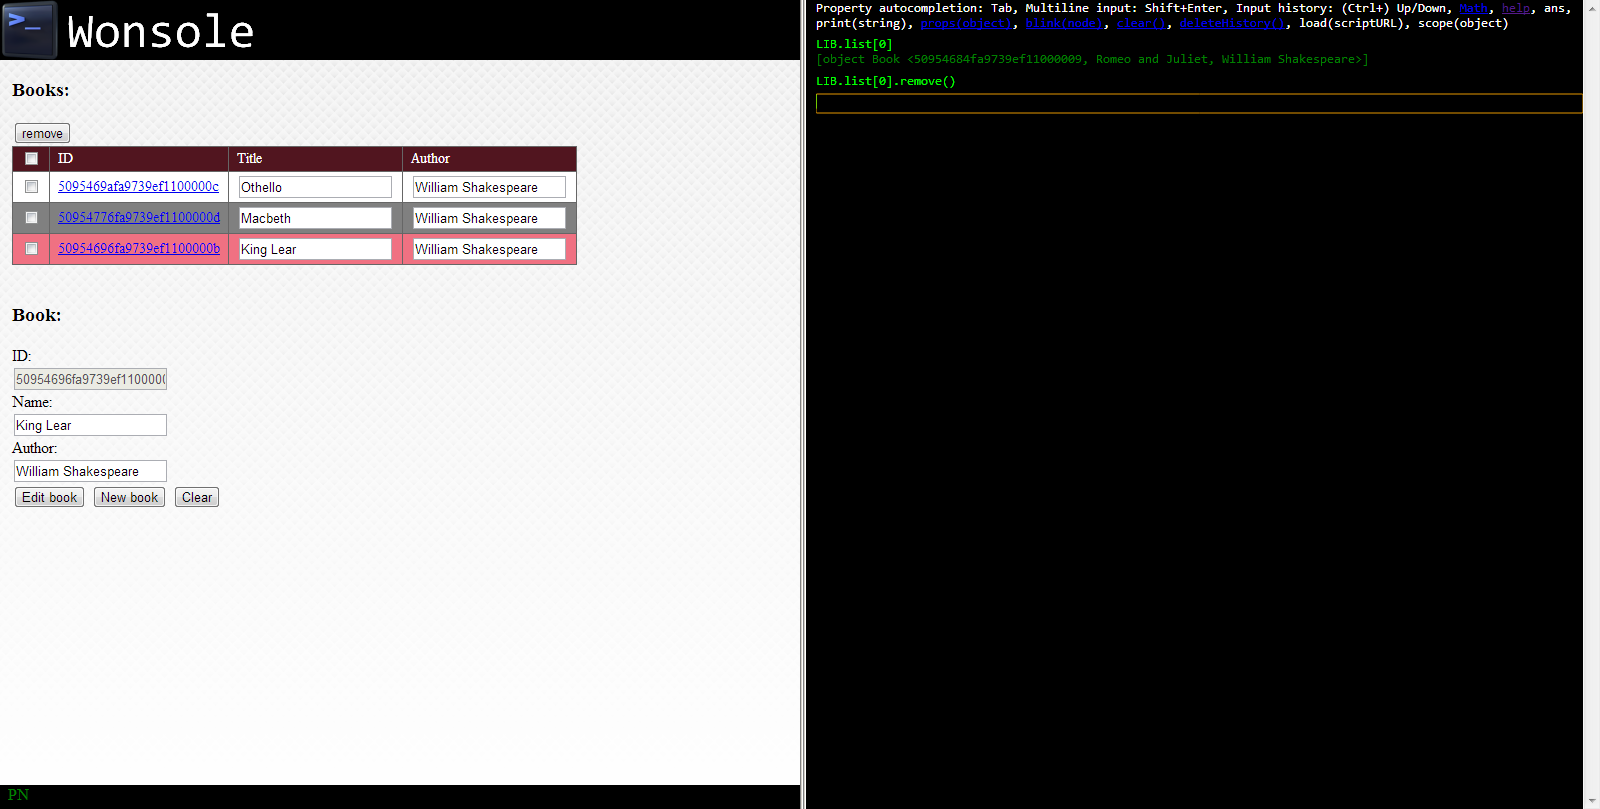
\includegraphics[width=\textwidth]{screenshot/wonsole1-11-delete2.png}
\caption{wonsole1-11-delete2.png}
\label{wonsole1-11-delete2.png}
\end{figure}


\begin{figure}
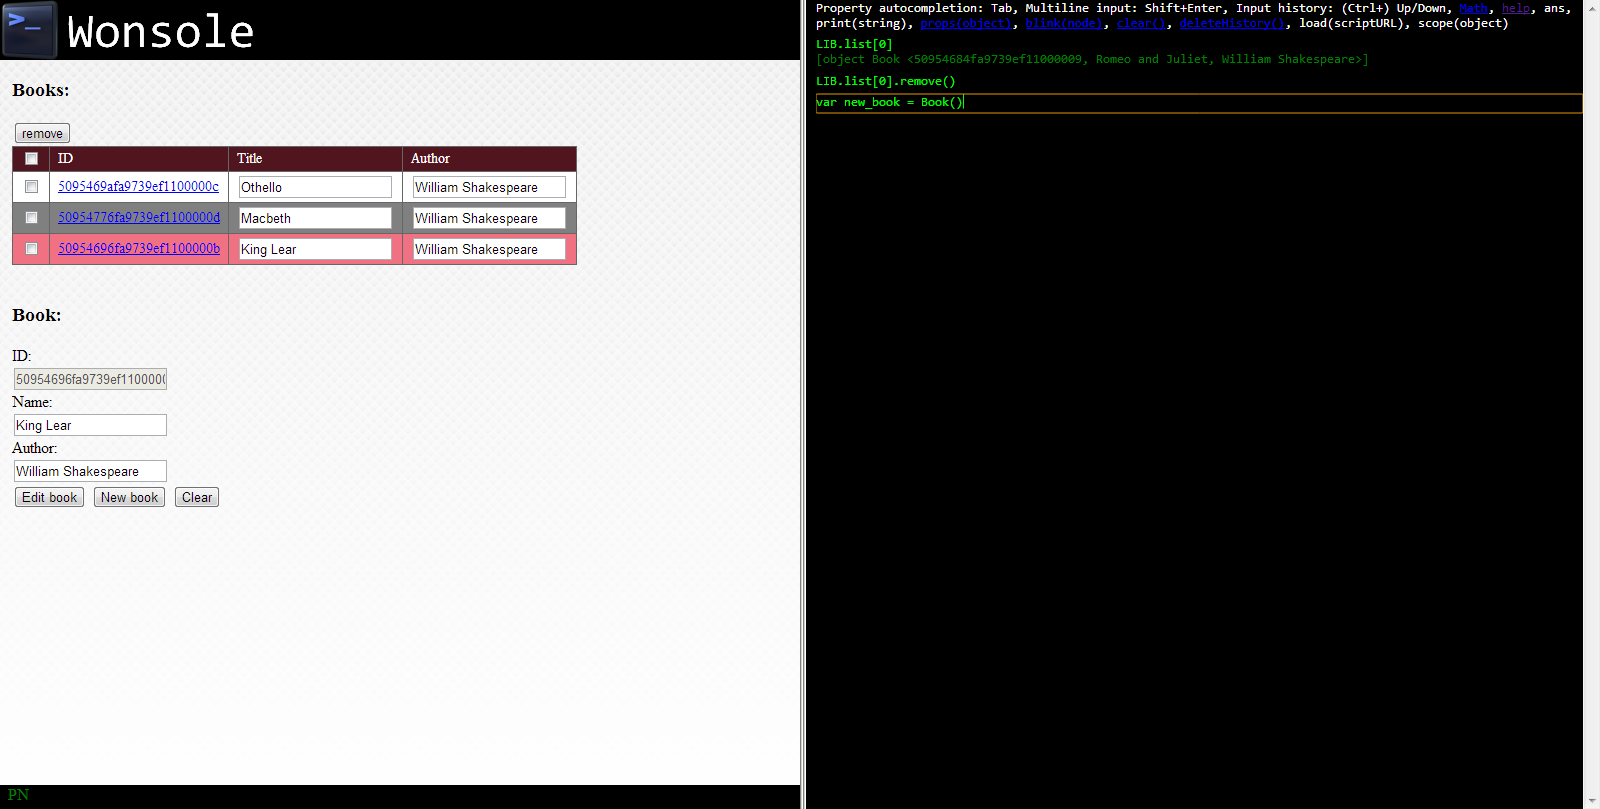
\includegraphics[width=\textwidth]{screenshot/wonsole1-12-new.png}
\caption{wonsole1-12-new.png}
\label{wonsole1-12-new.png}
\end{figure}


\clearpage
\begin{figure}
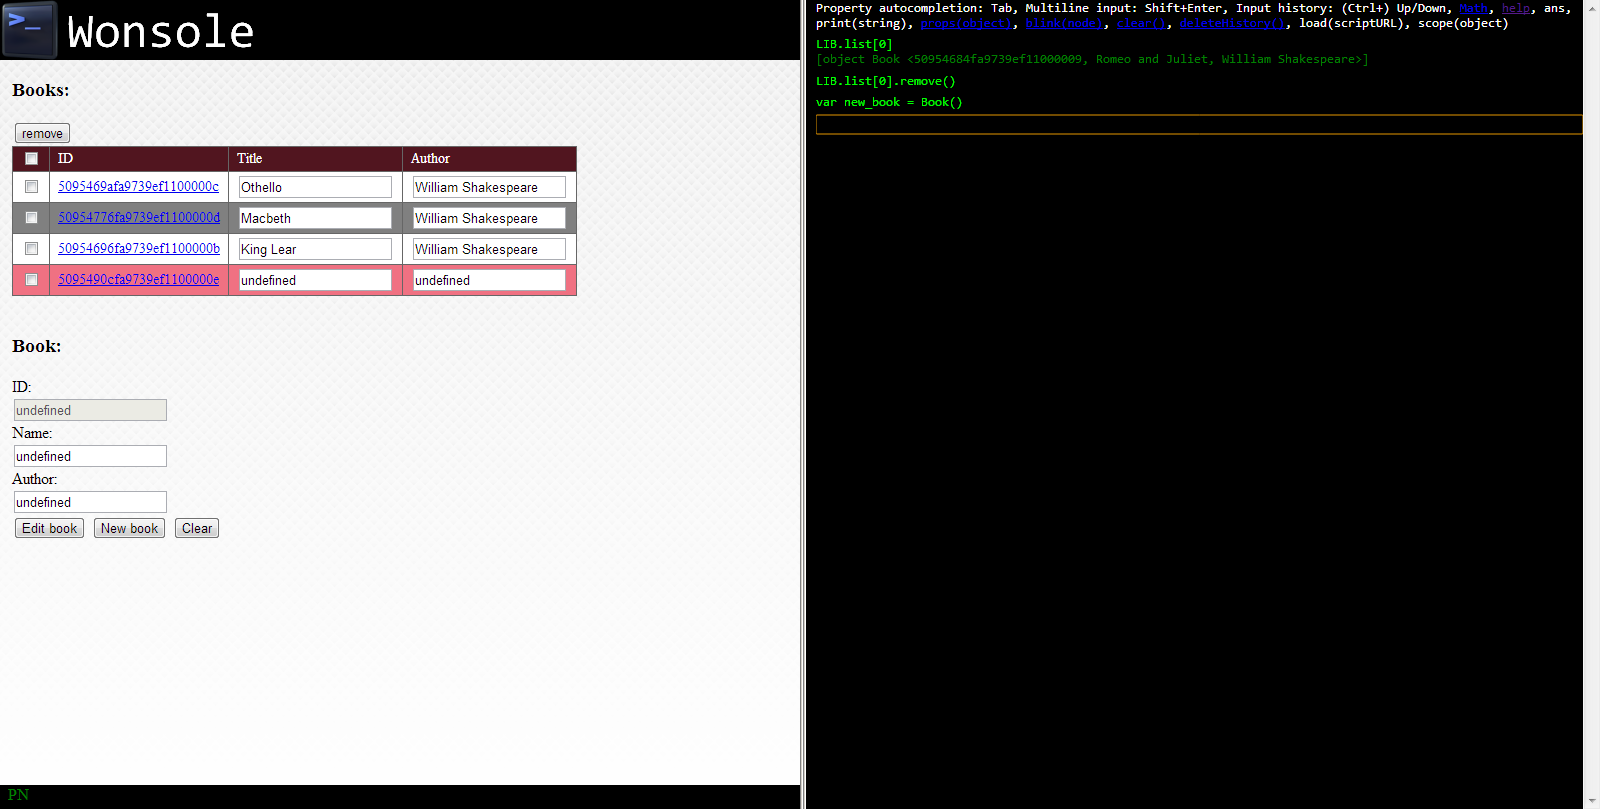
\includegraphics[width=\textwidth]{screenshot/wonsole1-13-new2.png}
\caption{wonsole1-13-new2.png}
\label{wonsole1-13-new2.png}
\end{figure}


\begin{figure}
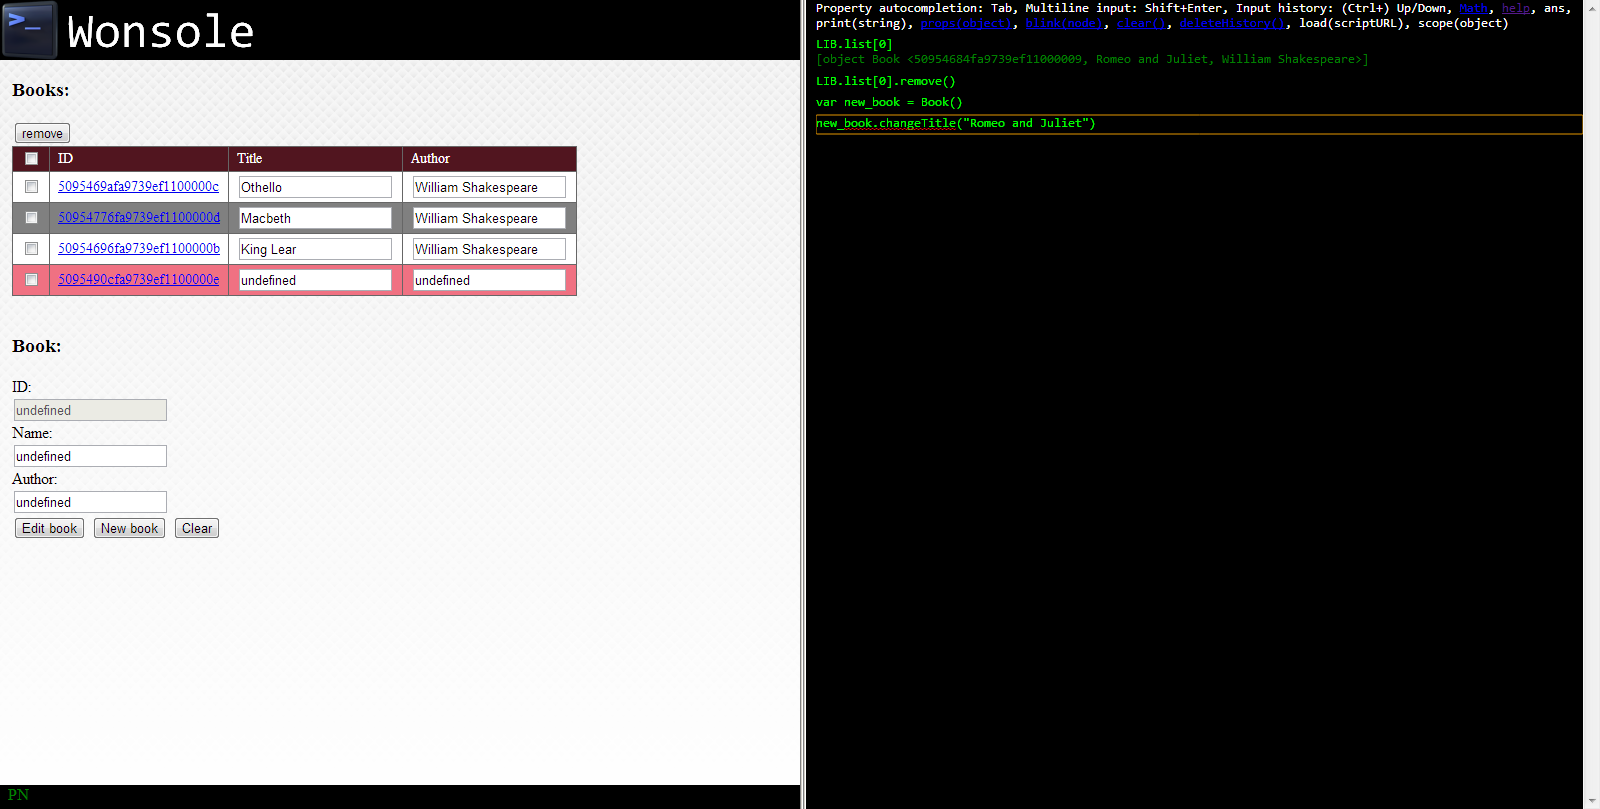
\includegraphics[width=\textwidth]{screenshot/wonsole1-14-title.png}
\caption{wonsole1-14-title.png}
\label{wonsole1-14-title.png}
\end{figure}


\clearpage
\begin{figure}
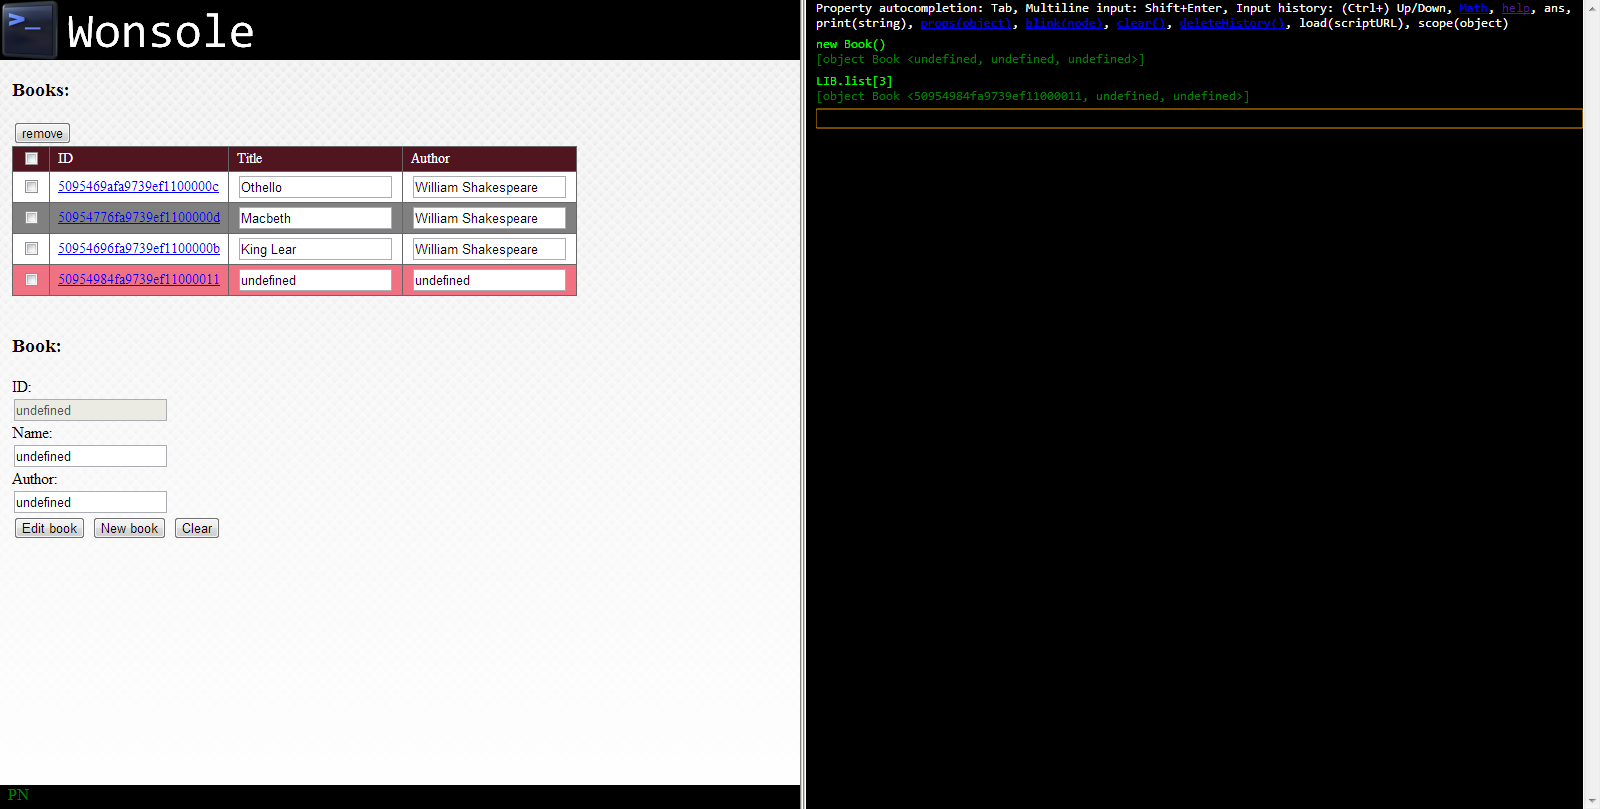
\includegraphics[width=\textwidth]{screenshot/wonsole1-15-title.png}
\caption{wonsole1-15-title.png}
\label{wonsole1-15-title.png}
\end{figure}


\begin{figure}
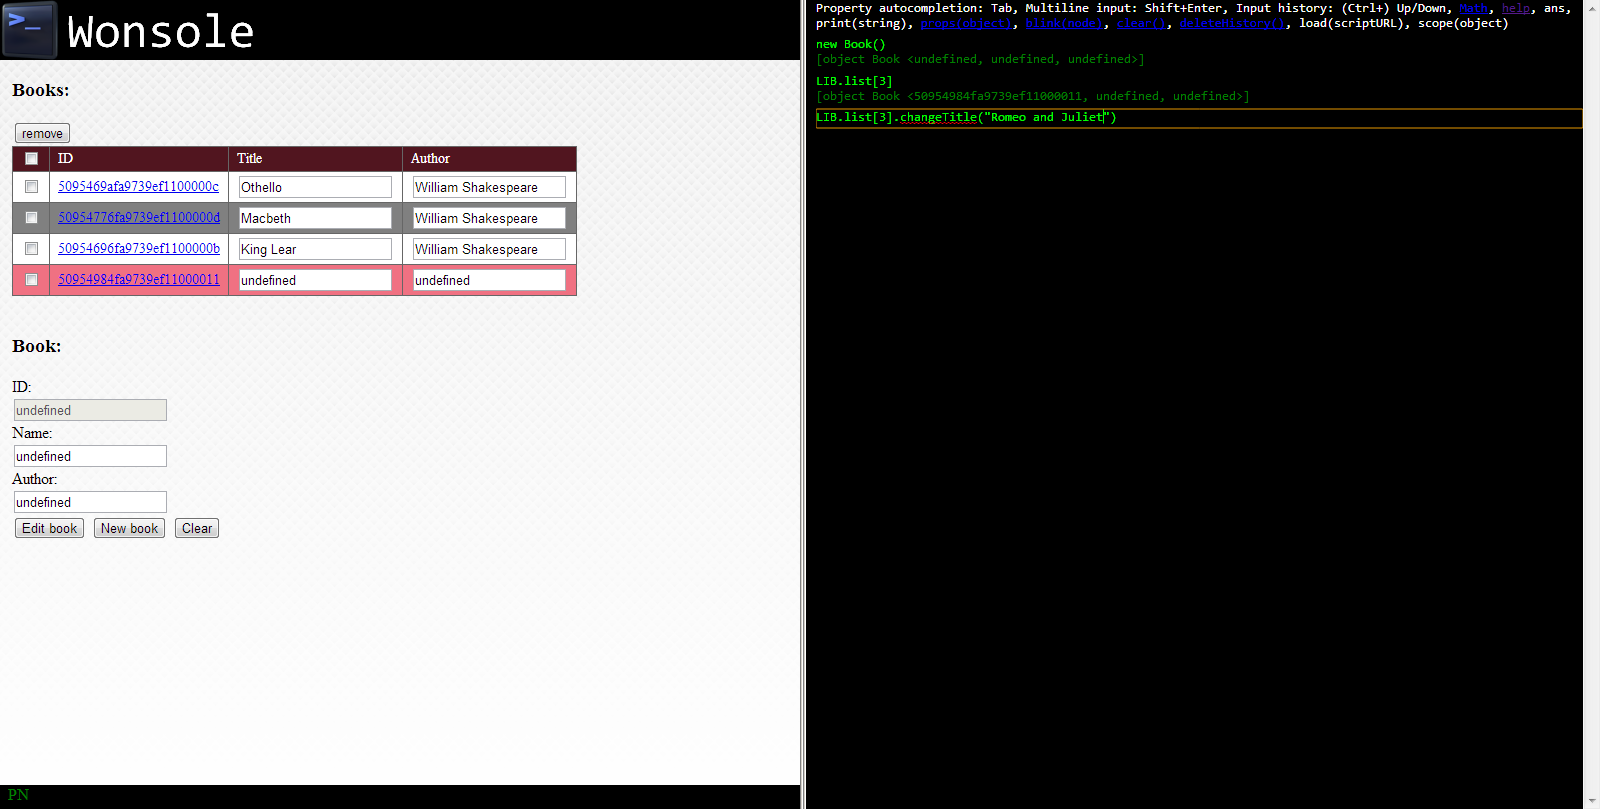
\includegraphics[width=\textwidth]{screenshot/wonsole1-16-title.png}
\caption{wonsole1-16-title.png}
\label{wonsole1-16-title.png}
\end{figure}


\clearpage
\begin{figure}
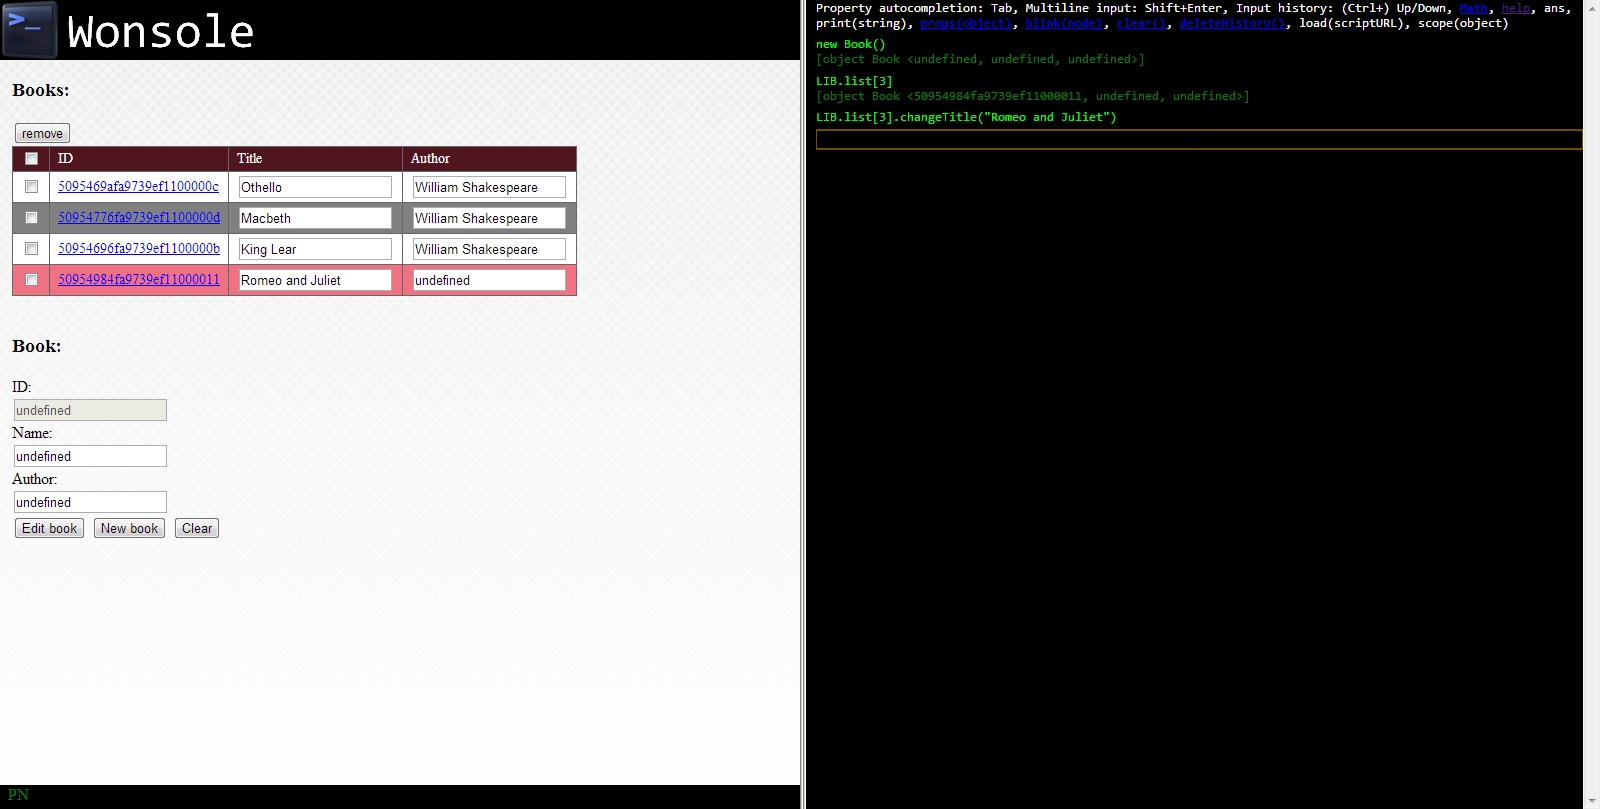
\includegraphics[width=\textwidth]{screenshot/wonsole1-17-title.png}
\caption{wonsole1-17-title.png}
\label{wonsole1-17-title.png}
\end{figure}


\begin{figure}
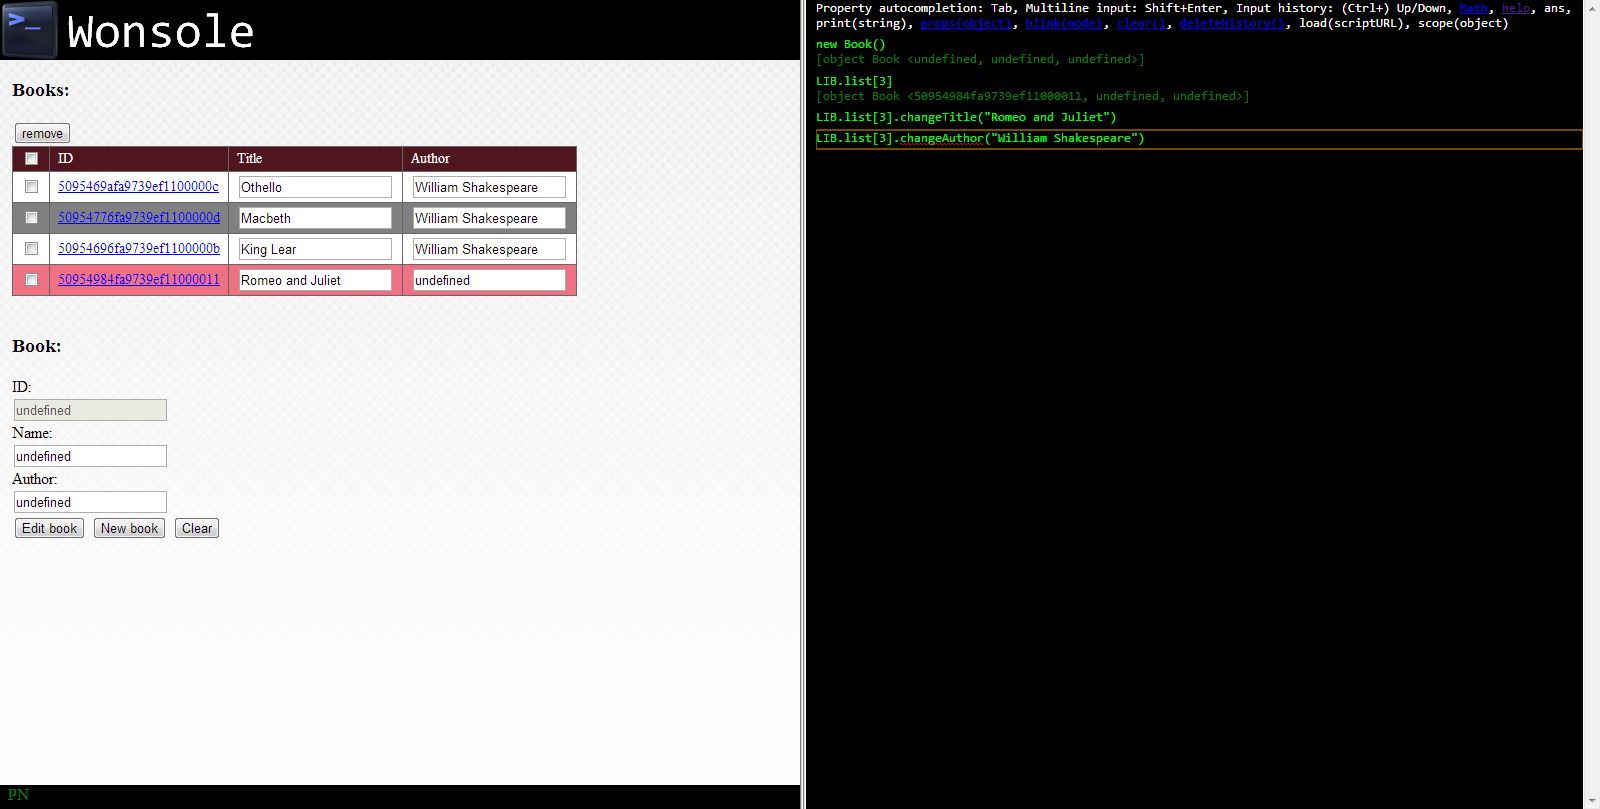
\includegraphics[width=\textwidth]{screenshot/wonsole1-18-author.png}
\caption{wonsole1-18-author.png}
\label{wonsole1-18-author.png}
\end{figure}


\clearpage
\begin{figure}
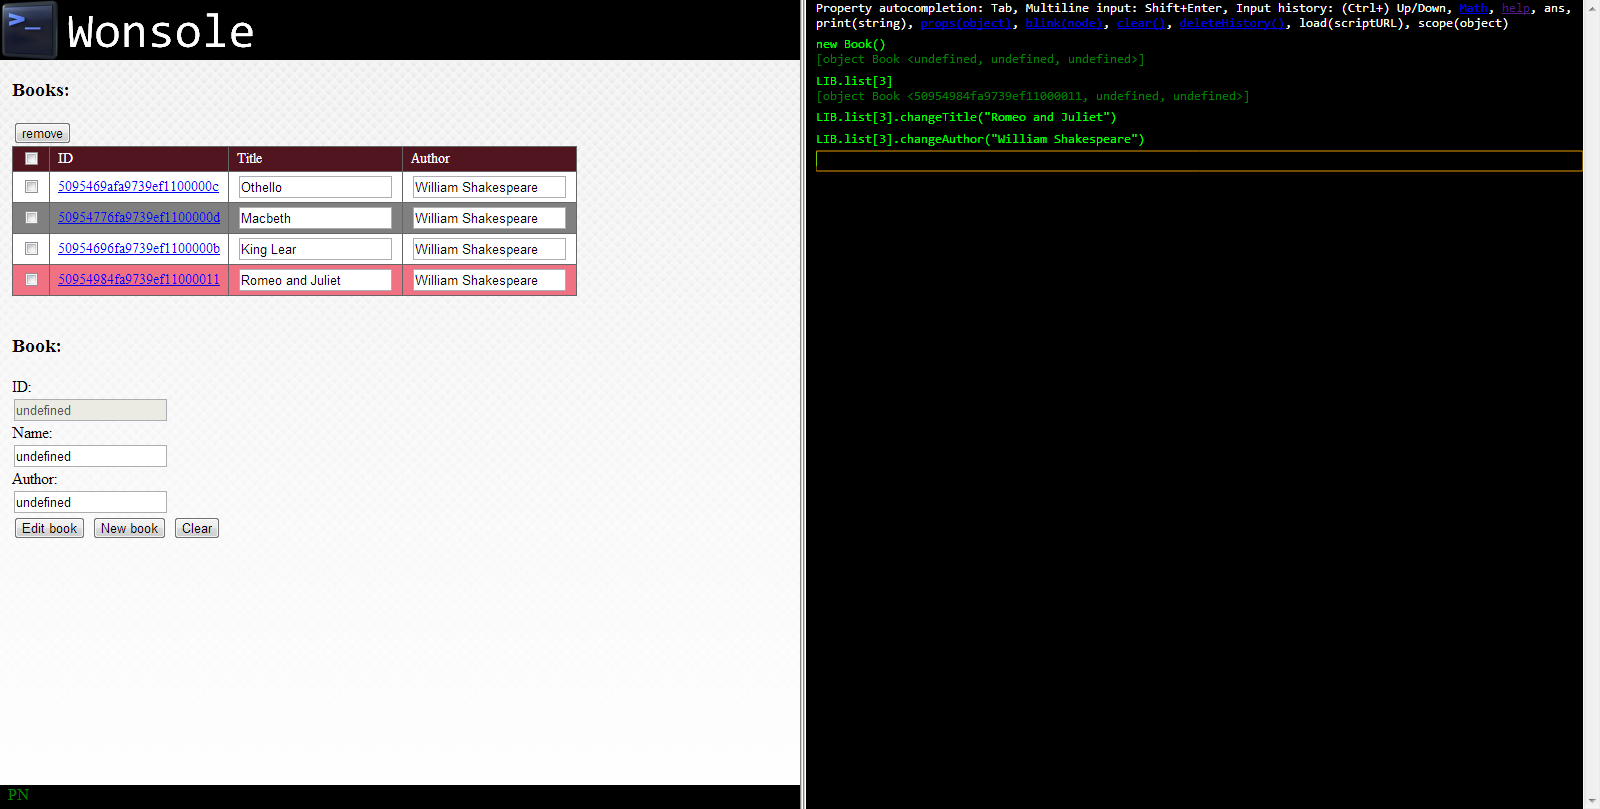
\includegraphics[width=\textwidth]{screenshot/wonsole1-19-author.png}
\caption{wonsole1-19-author.png}
\label{wonsole1-19-author.png}
\end{figure}


\begin{figure}
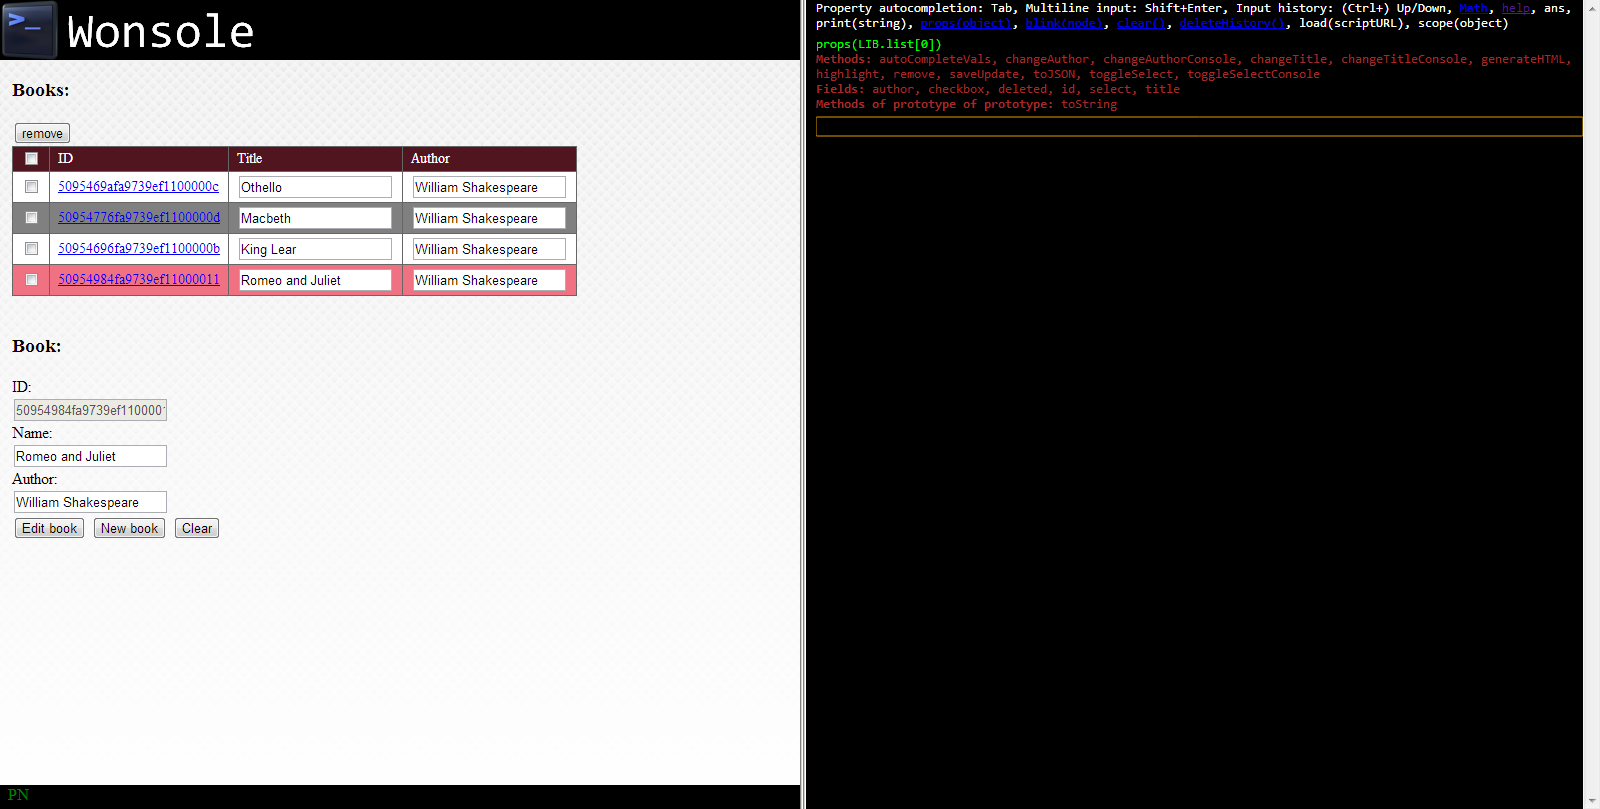
\includegraphics[width=\textwidth]{screenshot/wonsole1-20.png}
\caption{wonsole1-20.png}
\label{wonsole1-20.png}
\end{figure}


\clearpage
\begin{figure}
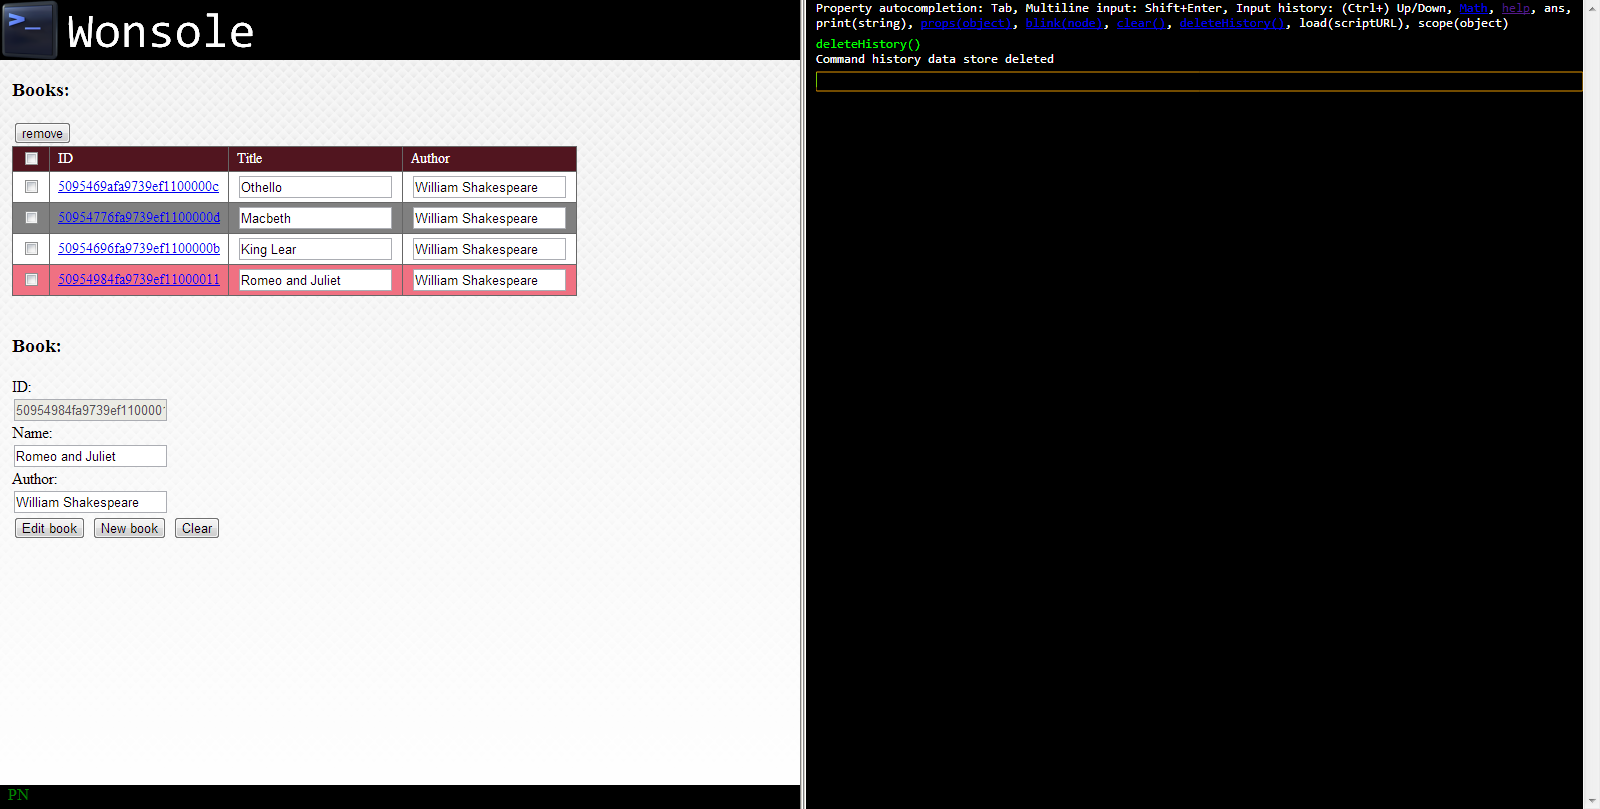
\includegraphics[width=\textwidth]{screenshot/wonsole1-21-delete-history.png}
\caption{wonsole1-21-delete-history.png}
\label{wonsole1-21-delete-history.png}
\end{figure}


\begin{figure}
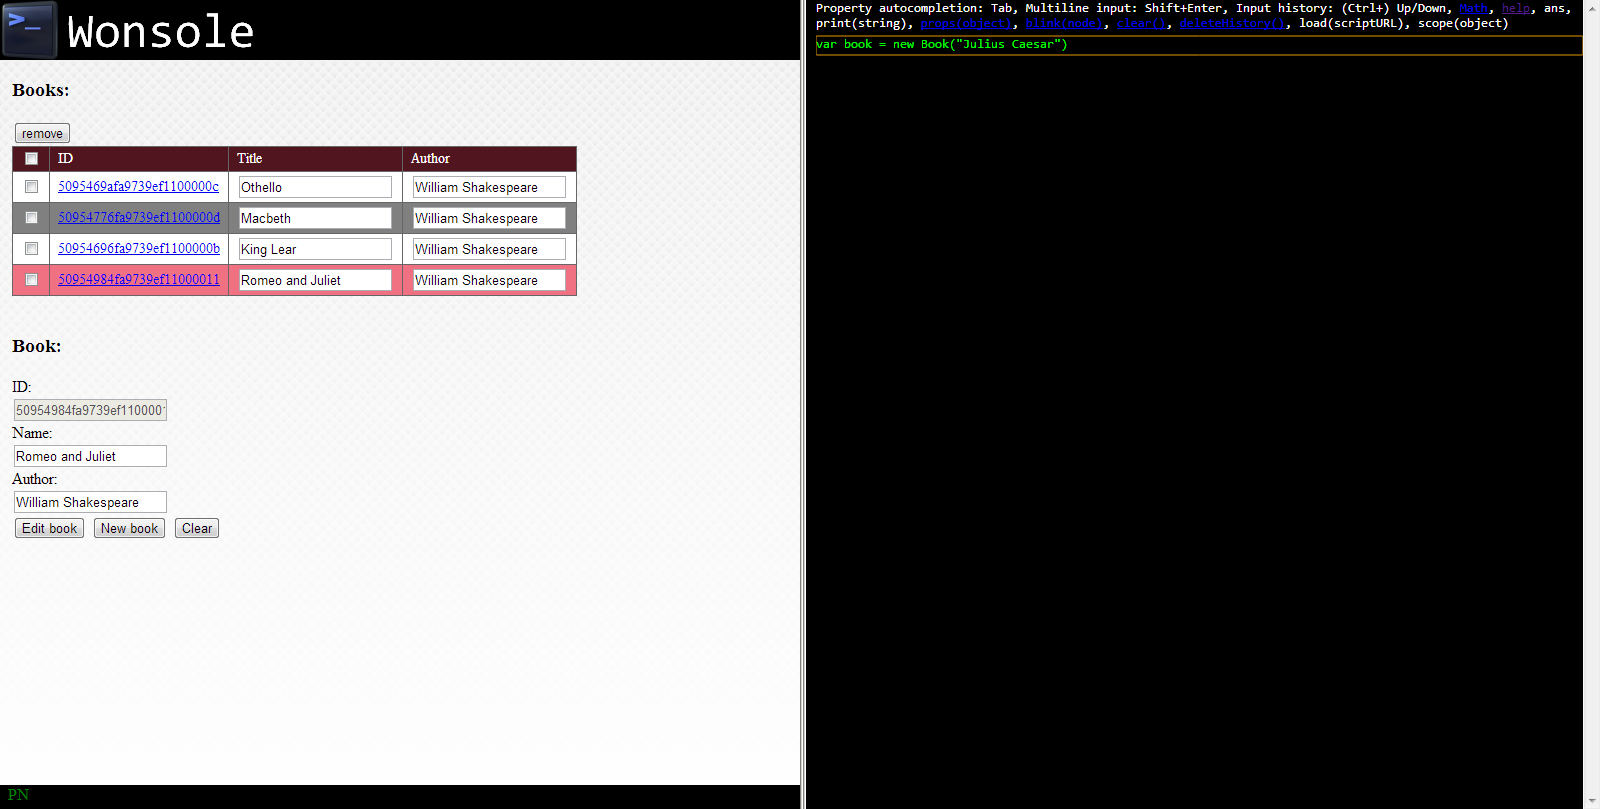
\includegraphics[width=\textwidth]{screenshot/wonsole1-22-new.png}
\caption{wonsole1-22-new.png}
\label{wonsole1-22-new.png}
\end{figure}


\clearpage
\begin{figure}
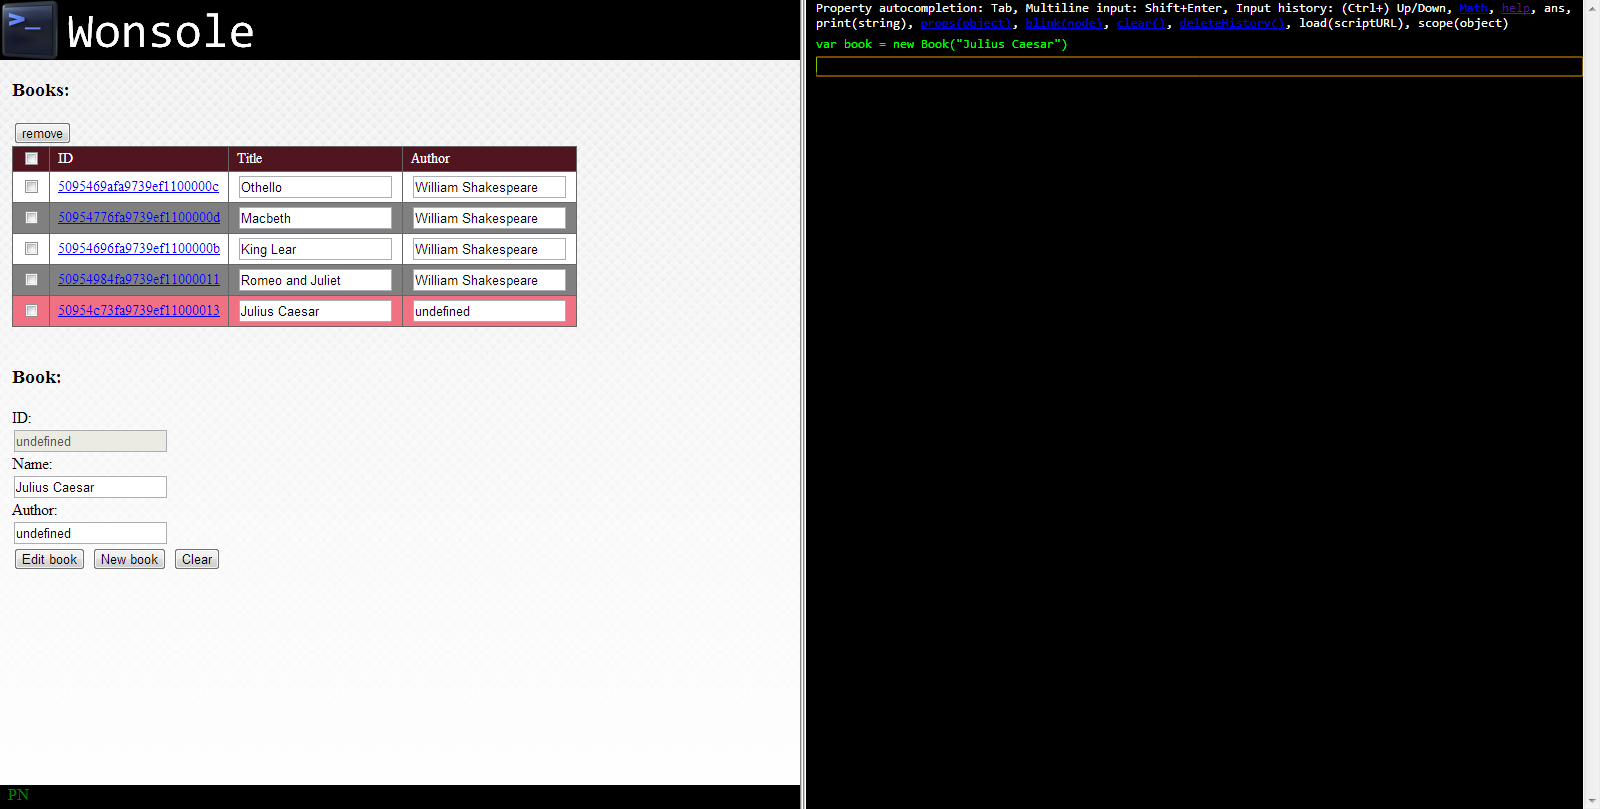
\includegraphics[width=\textwidth]{screenshot/wonsole1-23-new2.png}
\caption{wonsole1-23-new2.png}
\label{wonsole1-23-new2.png}
\end{figure}


\begin{figure}
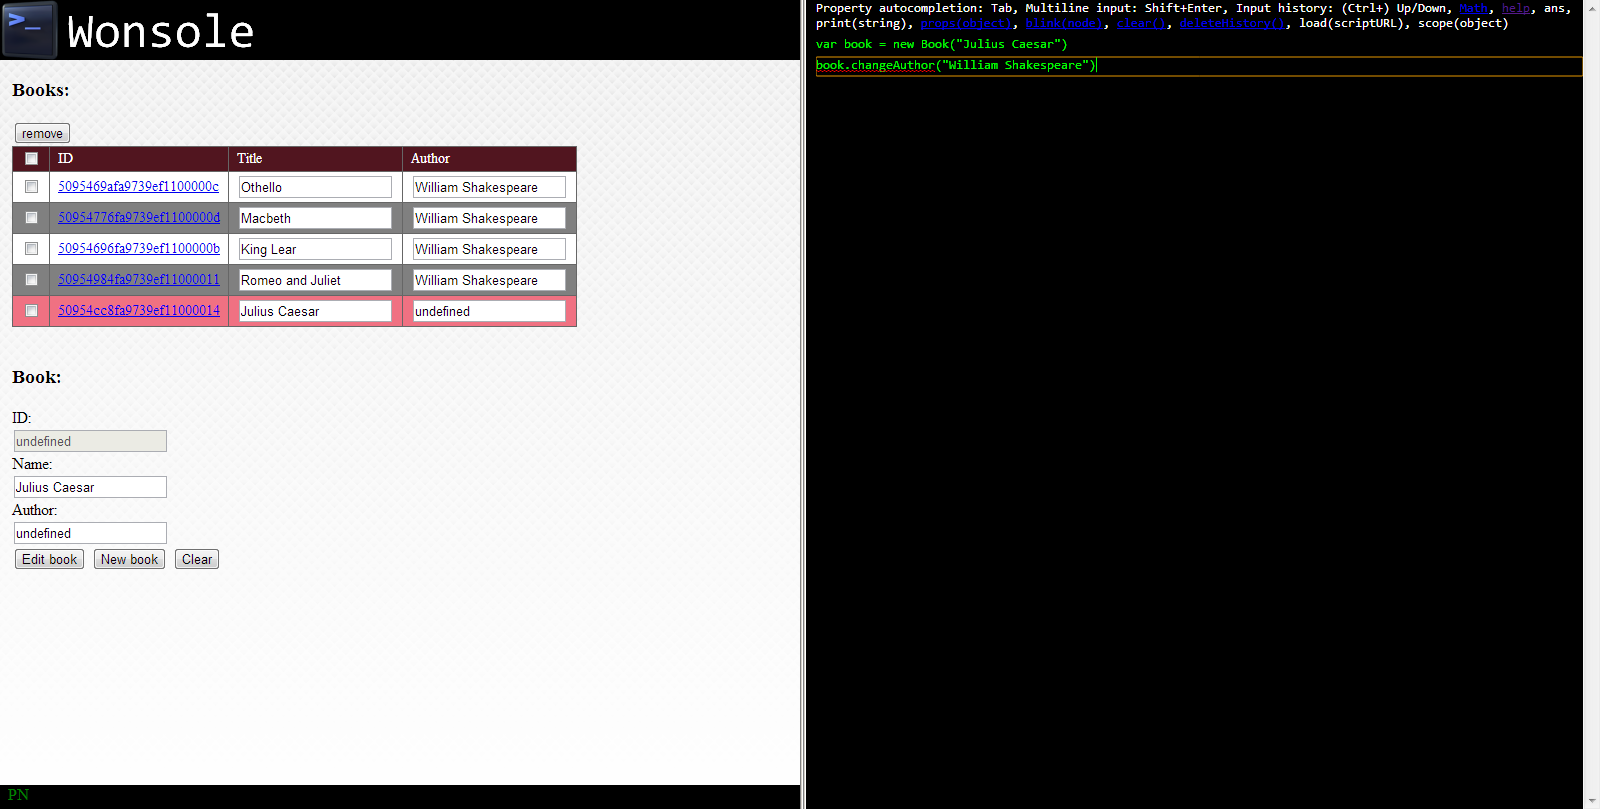
\includegraphics[width=\textwidth]{screenshot/wonsole1-24-author.png}
\caption{wonsole1-24-author.png}
\label{wonsole1-24-author.png}
\end{figure}


\clearpage
\begin{figure}
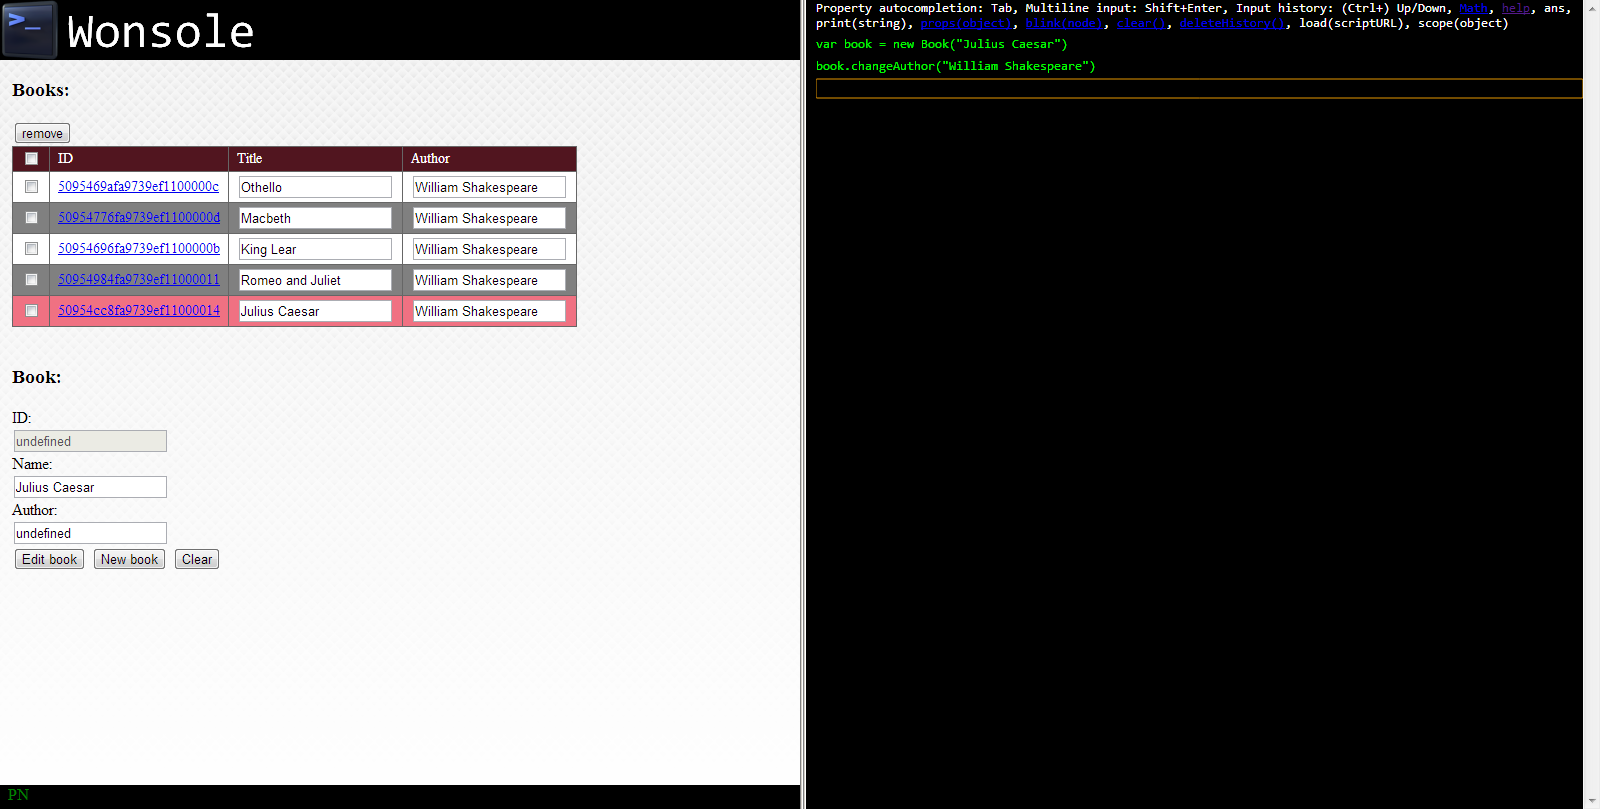
\includegraphics[width=\textwidth]{screenshot/wonsole1-25-author2.png}
\caption{wonsole1-25-author2.png}
\label{wonsole1-25-author2.png}
\end{figure}


\begin{figure}
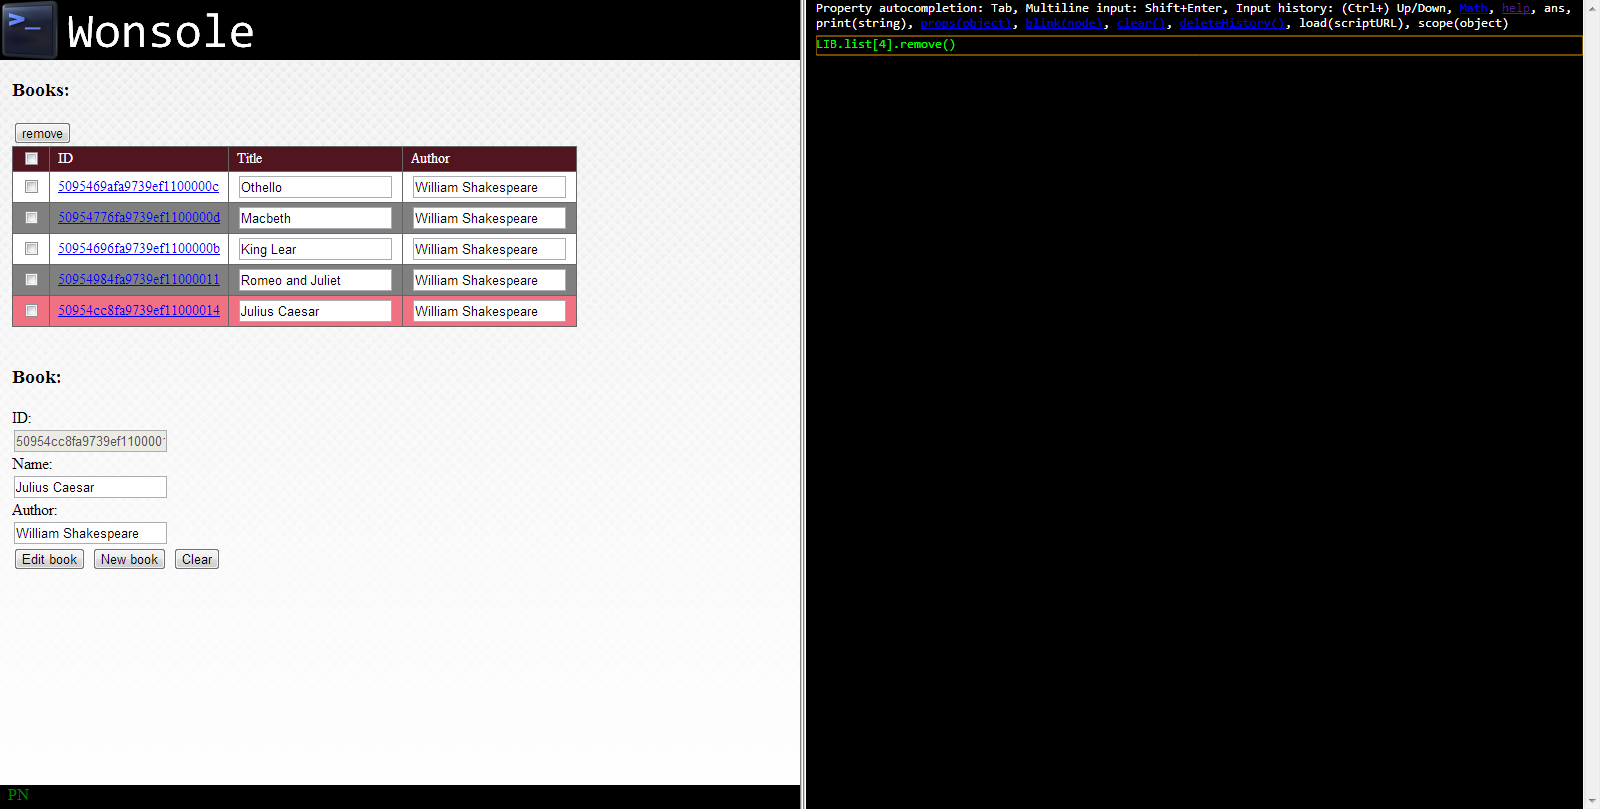
\includegraphics[width=\textwidth]{screenshot/wonsole1-26-remove.png}
\caption{wonsole1-26-remove.png}
\label{wonsole1-26-remove.png}
\end{figure}


\clearpage
\begin{figure}
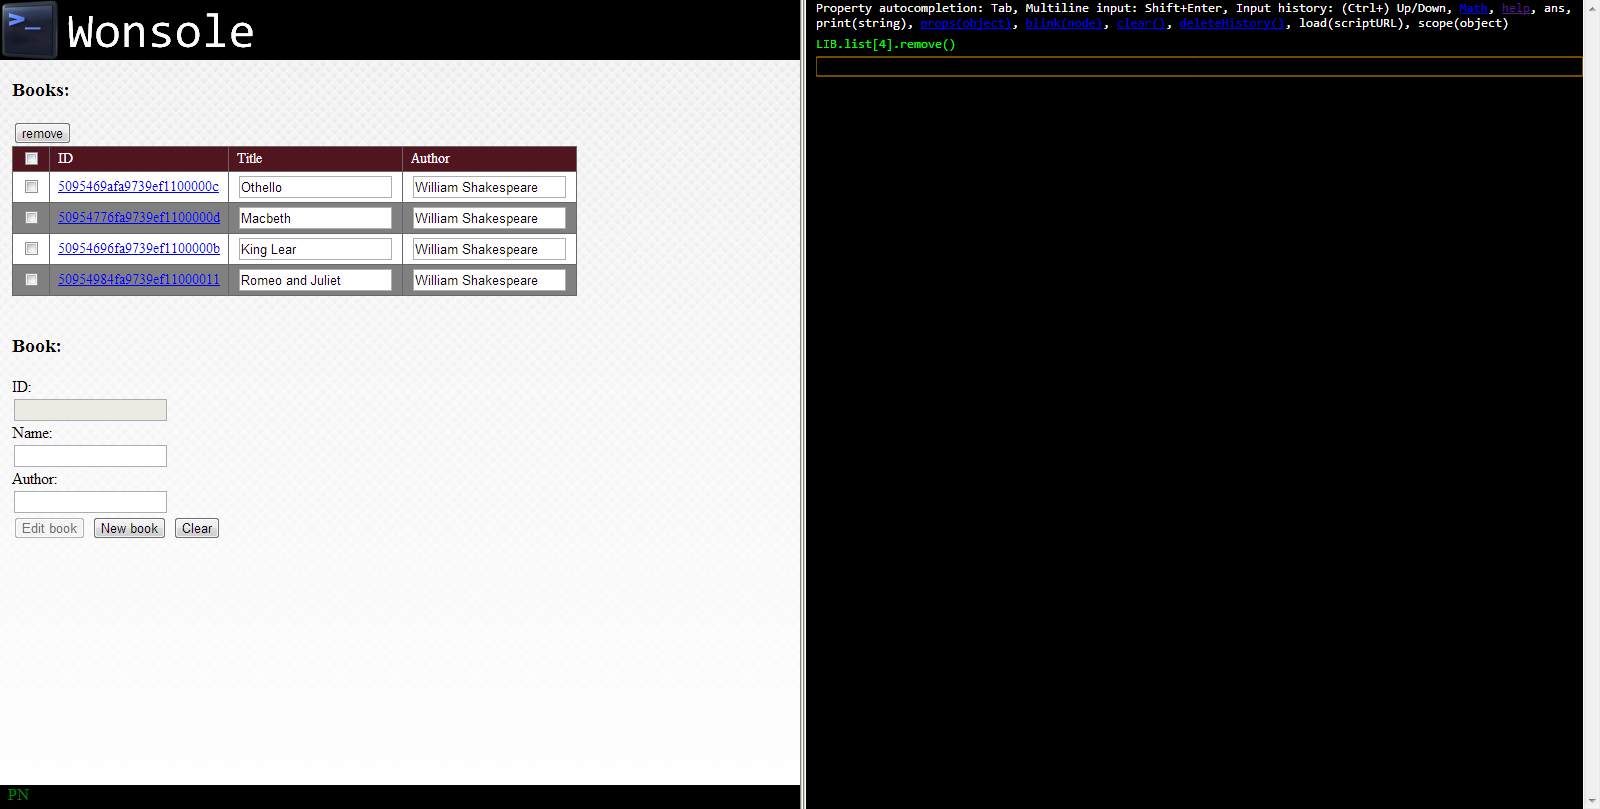
\includegraphics[width=\textwidth]{screenshot/wonsole1-27-remove.png}
\caption{wonsole1-27-remove.png}
\label{wonsole1-27-remove.png}
\end{figure}


\begin{figure}
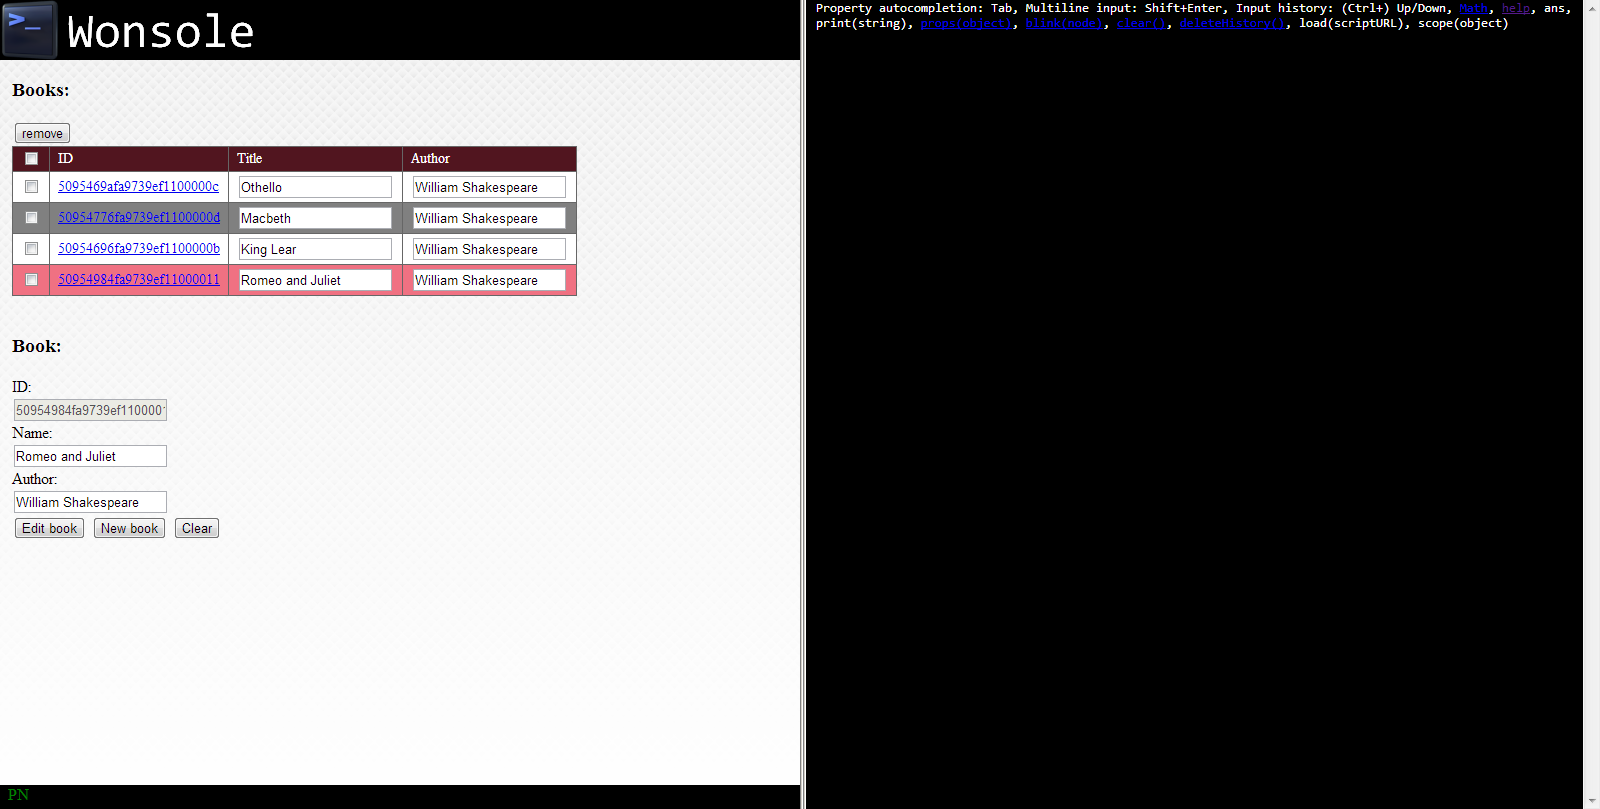
\includegraphics[width=\textwidth]{screenshot/wonsole1-28-remove.png}
\caption{wonsole1-28-remove.png}
\label{wonsole1-28-remove.png}
\end{figure}


\clearpage
\begin{figure}
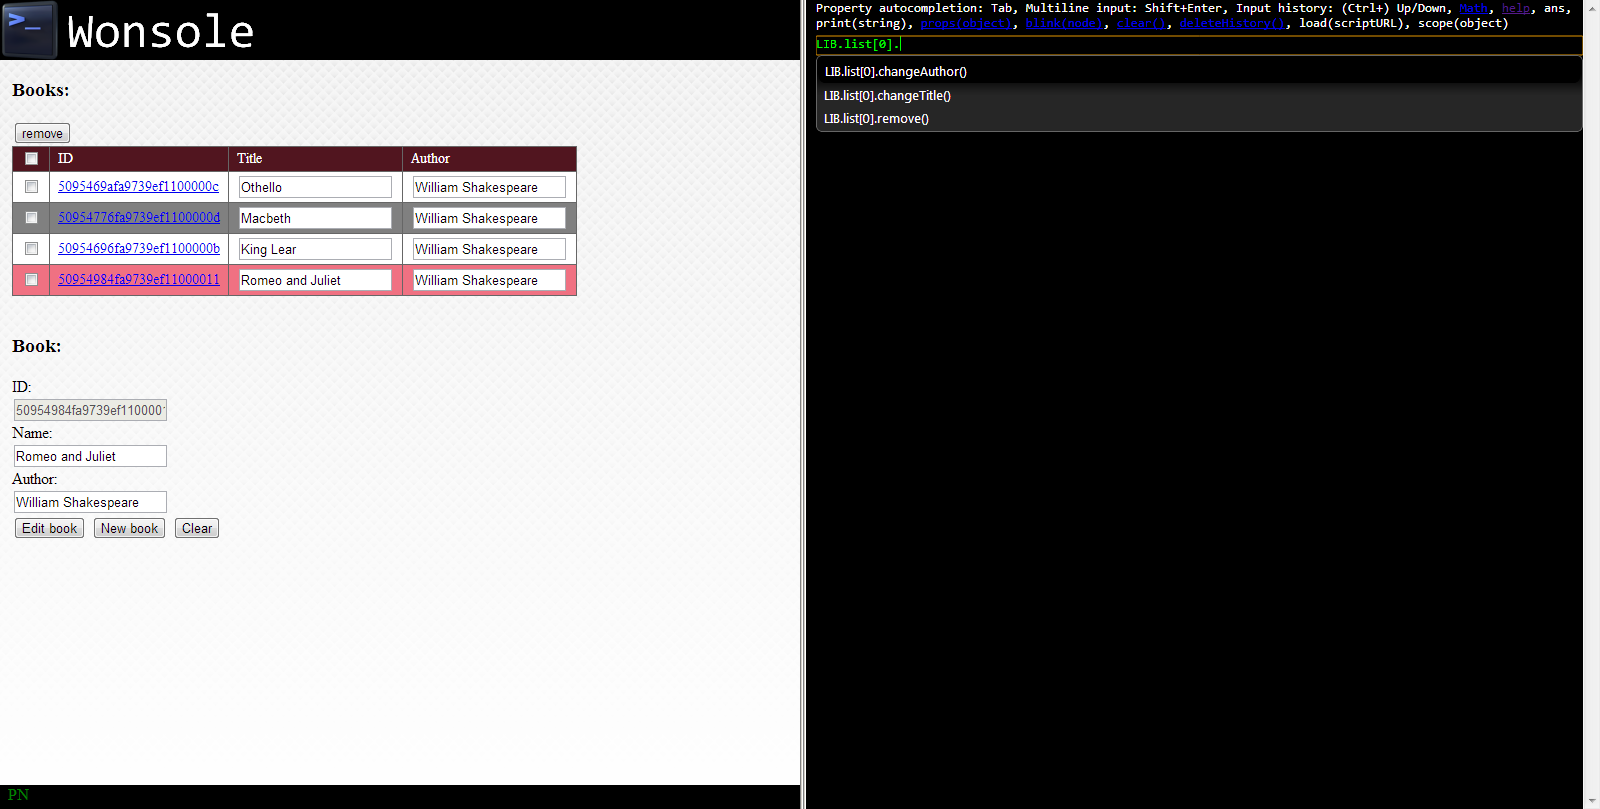
\includegraphics[width=\textwidth]{screenshot/wonsole1-29-autocompletion.png}
\caption{wonsole1-29-autocompletion.png}
\label{wonsole1-29-autocompletion.png}
\end{figure}


\begin{figure}
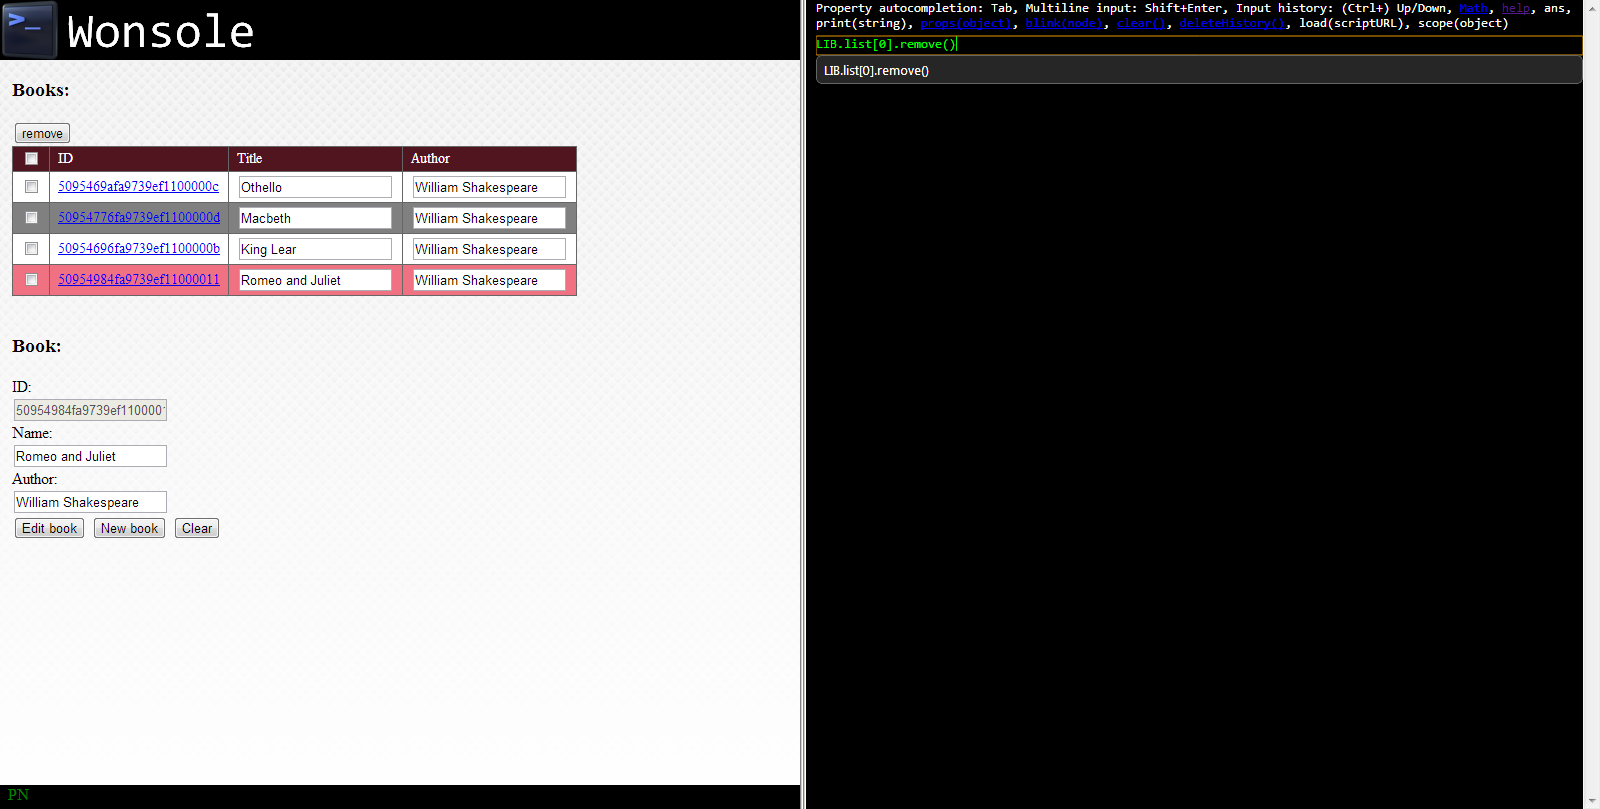
\includegraphics[width=\textwidth]{screenshot/wonsole1-30-autocompletion2.png}
\caption{wonsole1-30-autocompletion2.png}
\label{wonsole1-30-autocompletion2.png}
\end{figure}


\clearpage
\begin{figure}
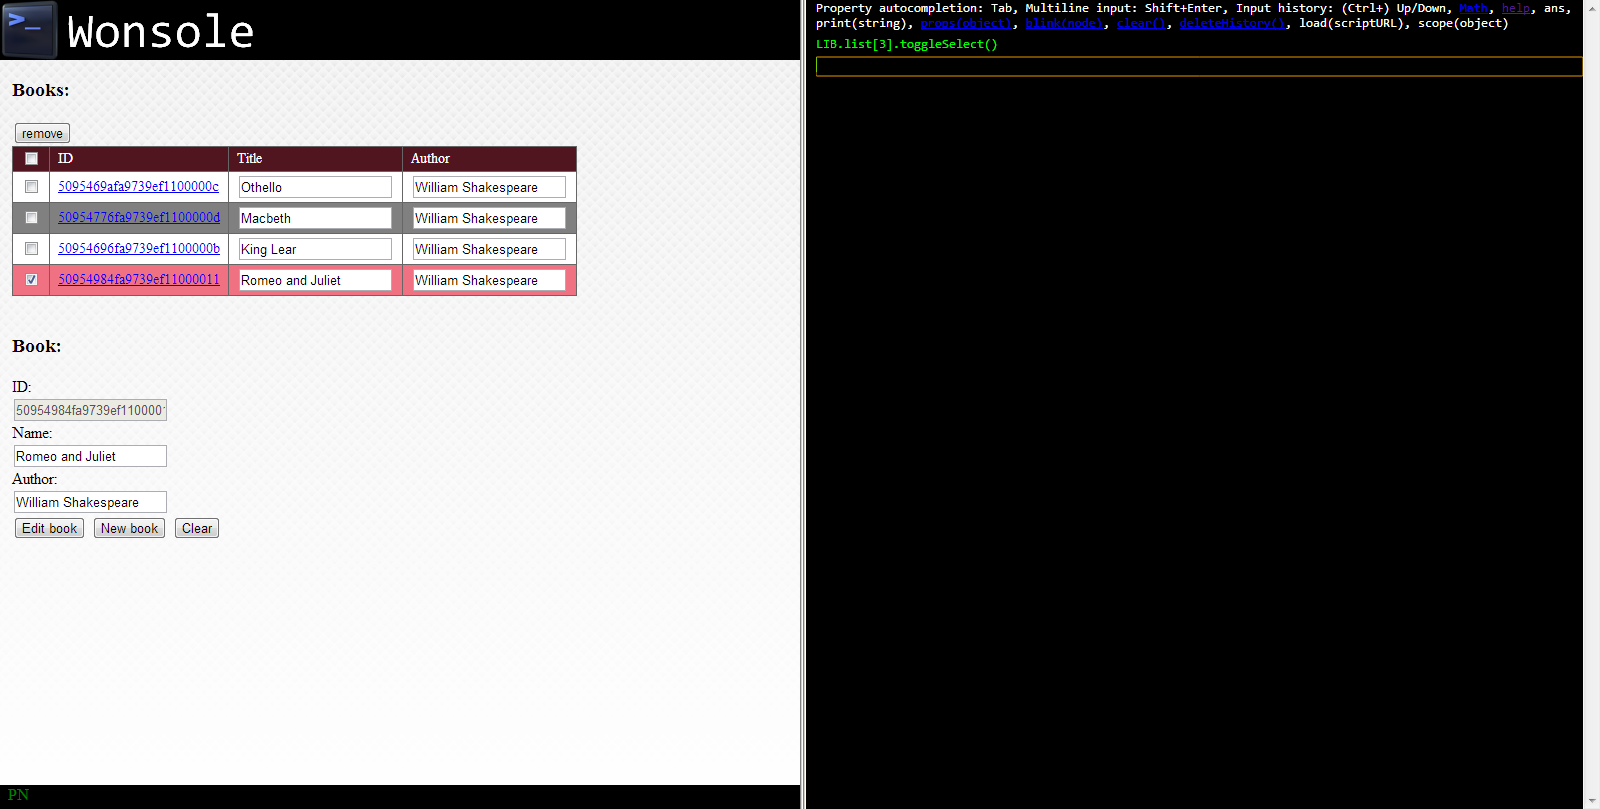
\includegraphics[width=\textwidth]{screenshot/wonsole1-31-select.png}
\caption{wonsole1-31-select.png}
\label{wonsole1-31-select.png}
\end{figure}


\begin{figure}
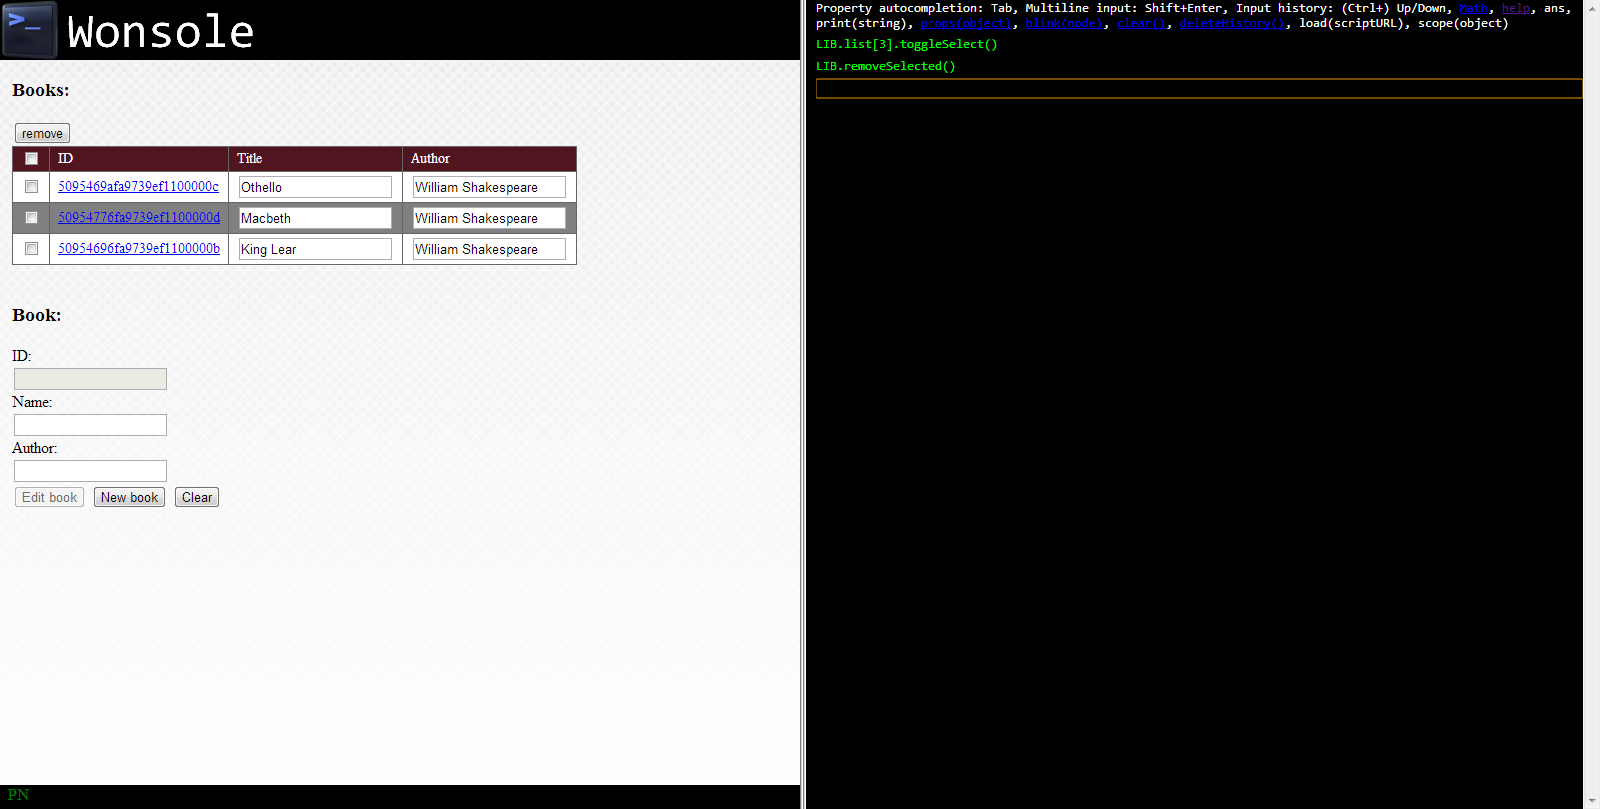
\includegraphics[width=\textwidth]{screenshot/wonsole1-32-remove.png}
\caption{wonsole1-32-remove.png}
\label{wonsole1-32-remove.png}
\end{figure}


\clearpage
\begin{figure}
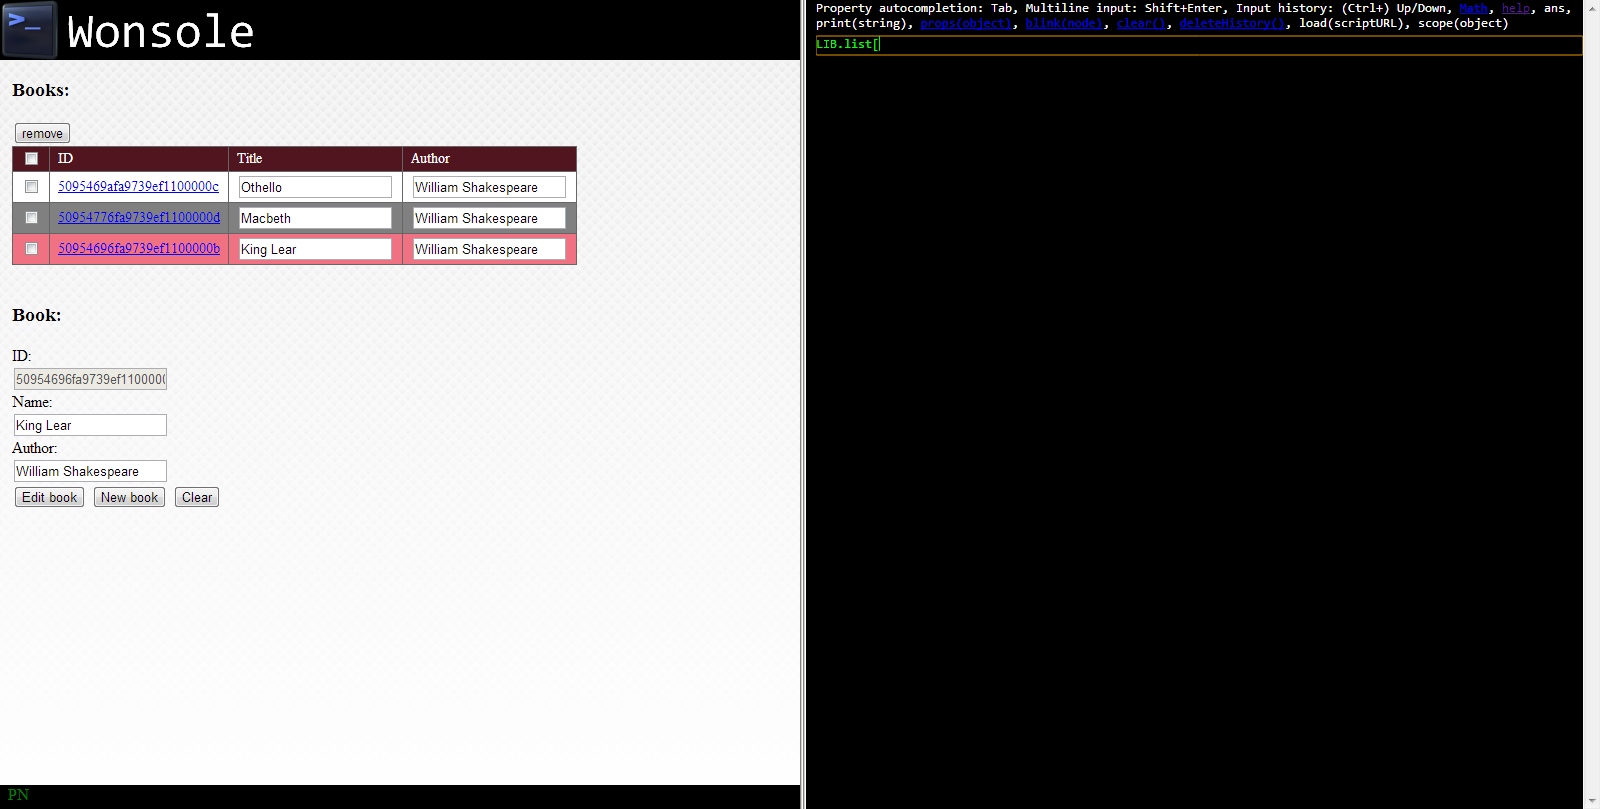
\includegraphics[width=\textwidth]{screenshot/wonsole1-33-tab.png}
\caption{wonsole1-33-tab.png}
\label{wonsole1-33-tab.png}
\end{figure}


\begin{figure}
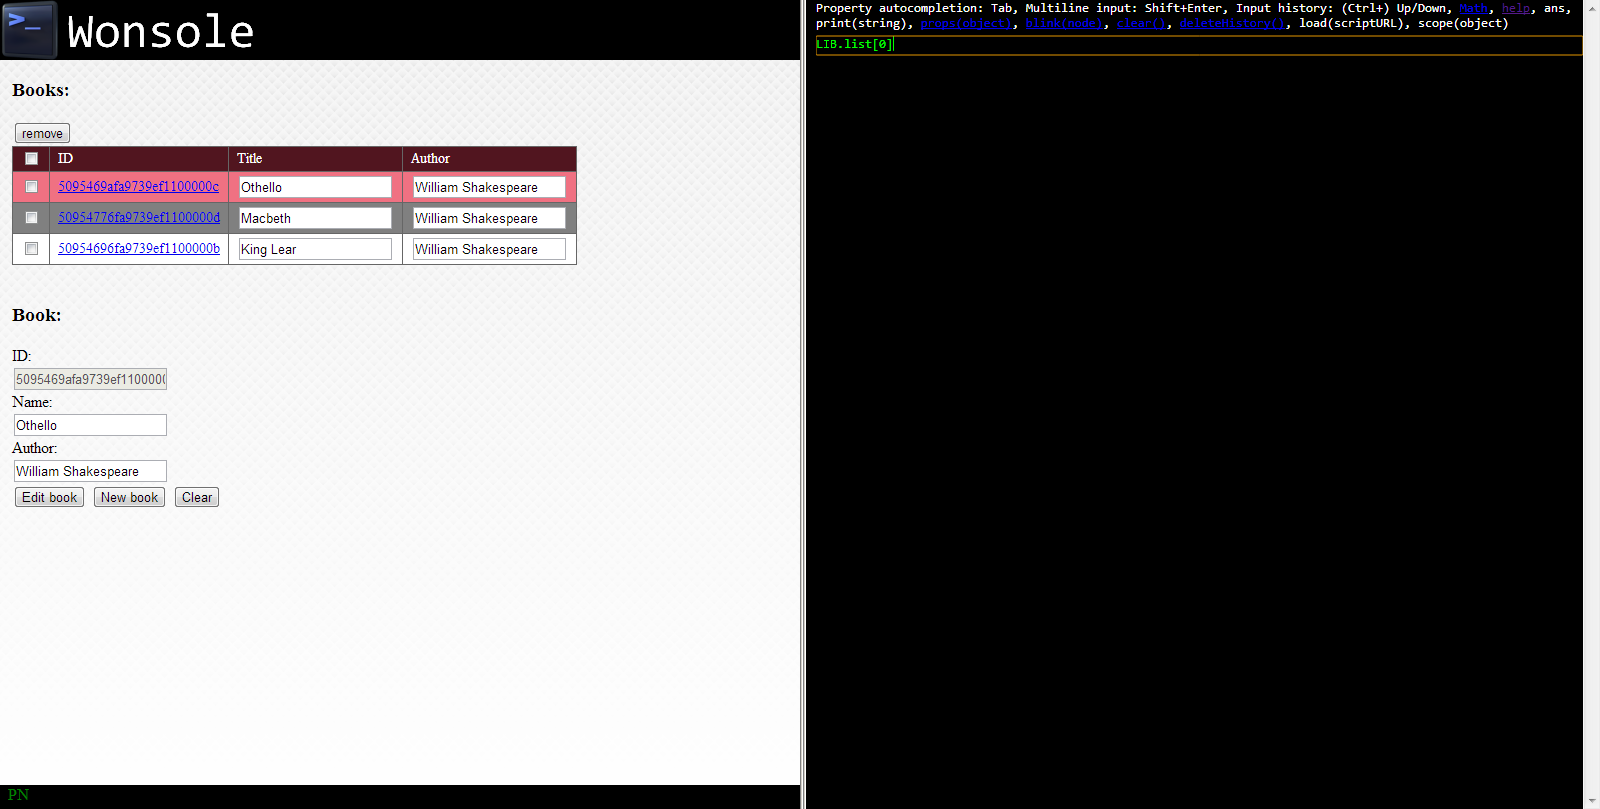
\includegraphics[width=\textwidth]{screenshot/wonsole1-34-tab.png}
\caption{wonsole1-34-tab.png}
\label{wonsole1-34-tab.png}
\end{figure}


\clearpage
\begin{figure}
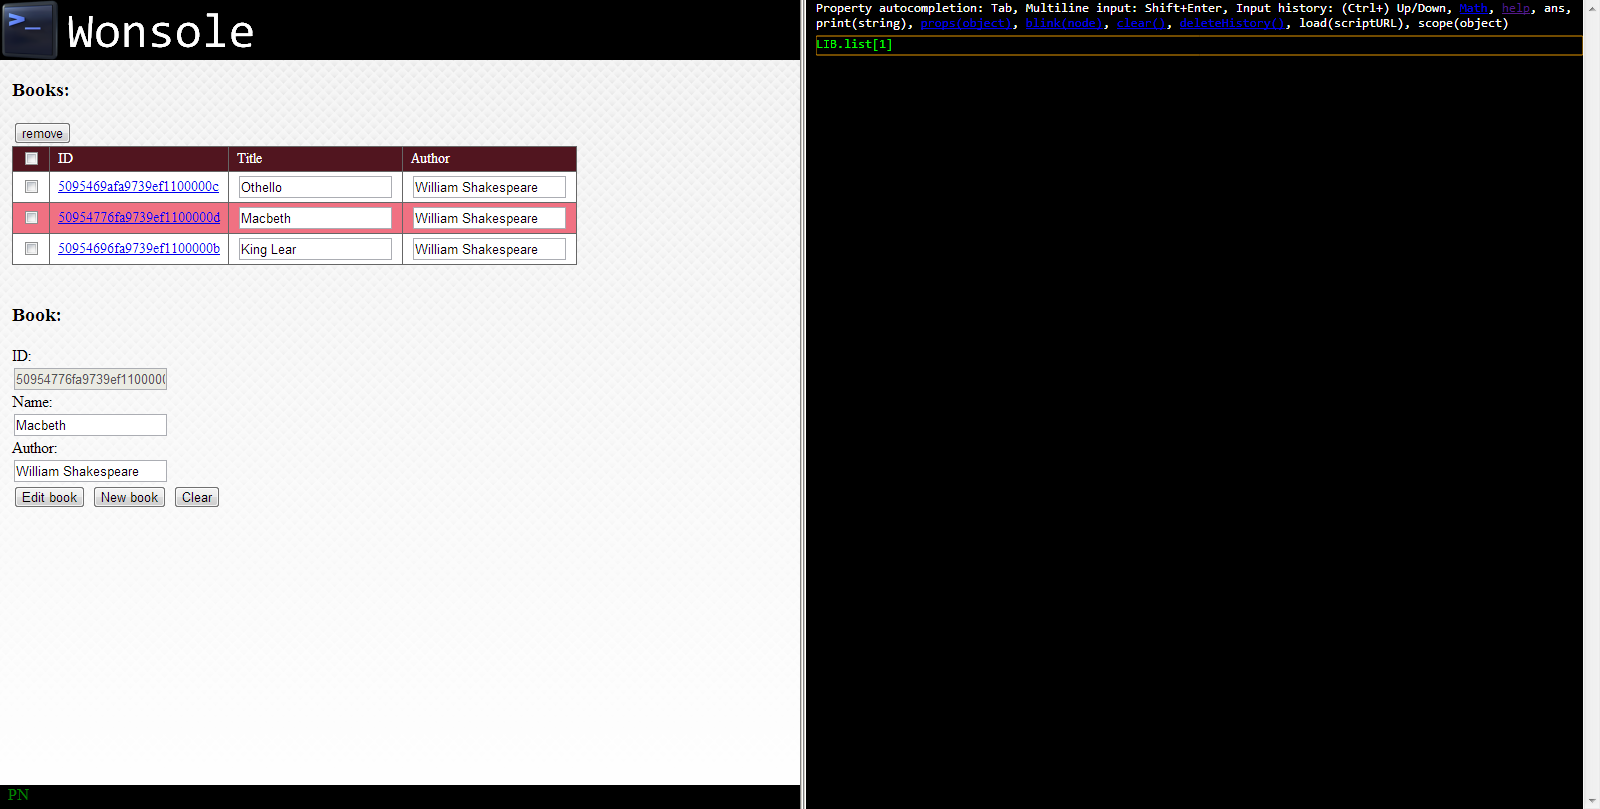
\includegraphics[width=\textwidth]{screenshot/wonsole1-35-tab.png}
\caption{wonsole1-35-tab.png}
\label{wonsole1-35-tab.png}
\end{figure}


\begin{figure}
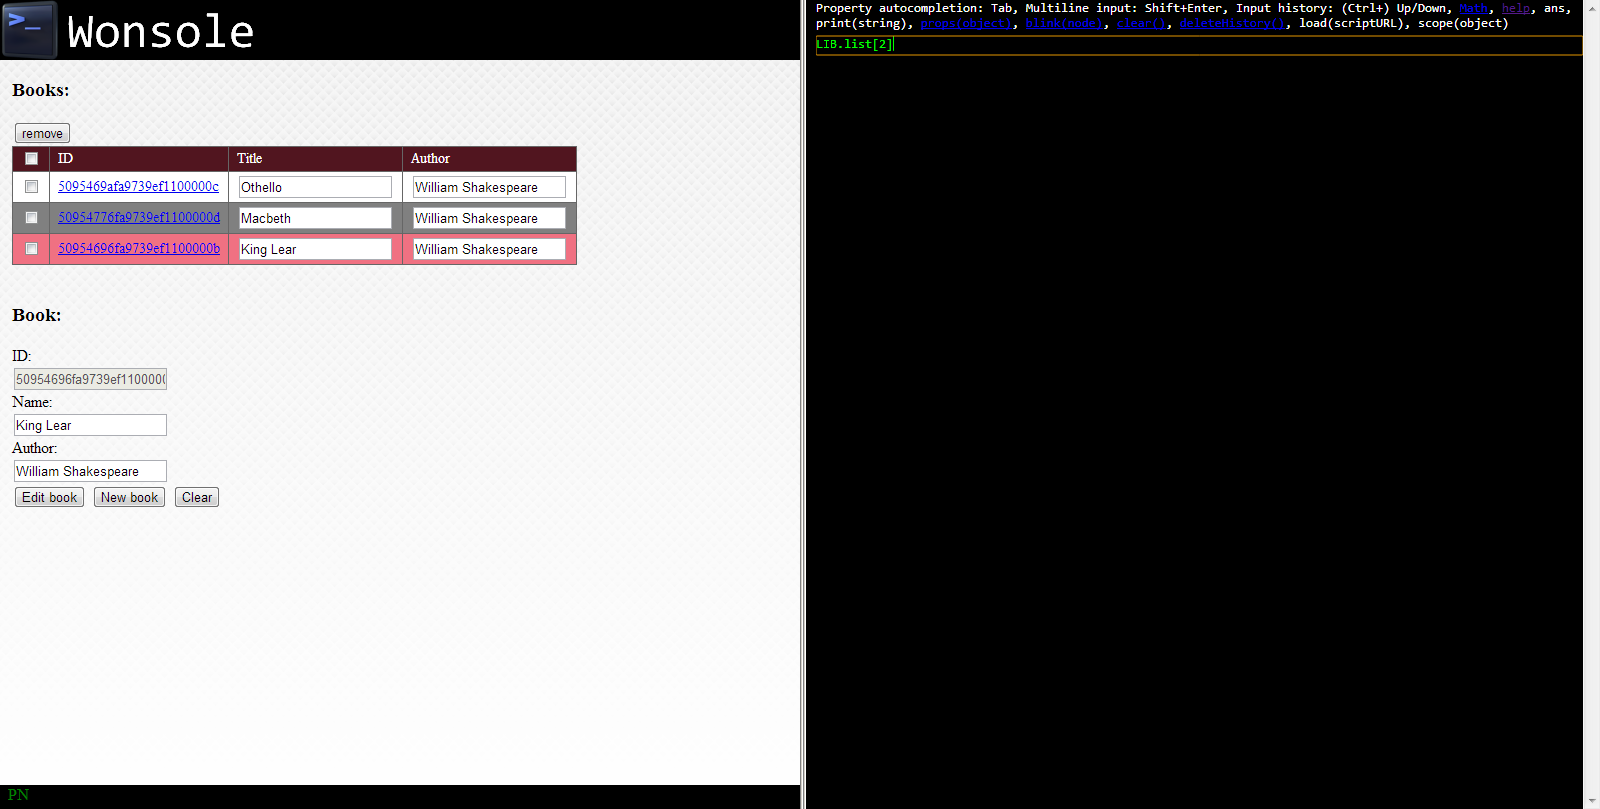
\includegraphics[width=\textwidth]{screenshot/wonsole1-36-tab.png}
\caption{wonsole1-36-tab.png}
\label{wonsole1-36-tab.png}
\end{figure}


\clearpage
\begin{figure}
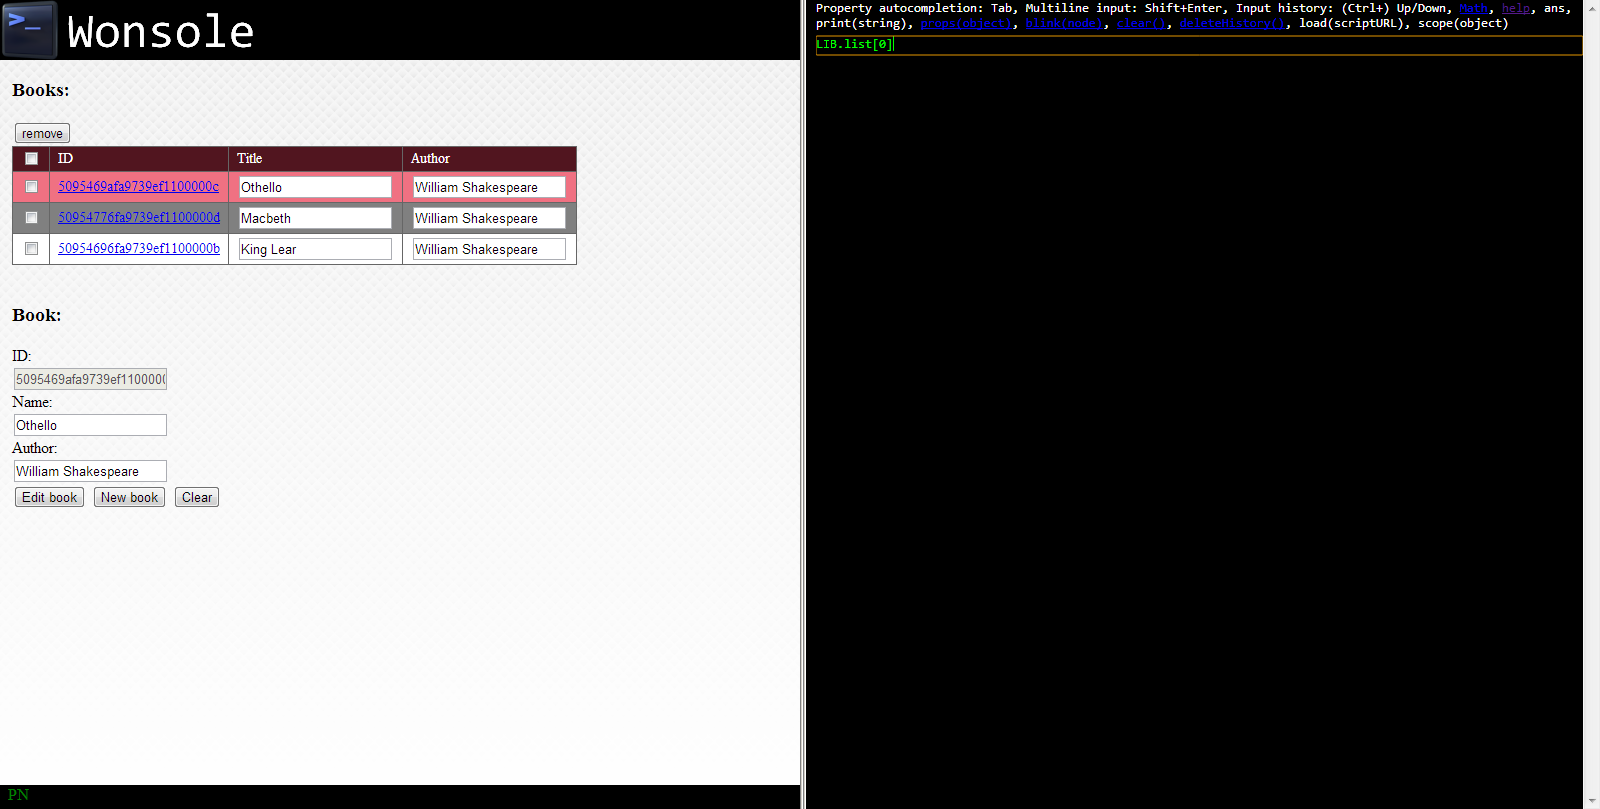
\includegraphics[width=\textwidth]{screenshot/wonsole1-37-tab.png}
\caption{wonsole1-37-tab.png}
\label{wonsole1-37-tab.png}
\end{figure}



\end{document}
